%% LaTeX2e class for student theses
%% thesis.tex
%% 
%% Karlsruhe Institute of Technology
%% Institute for Program Structures and Data Organization
%% Chair for Software Design and Quality (SDQ)
%%
%% Dr.-Ing. Erik Burger
%% burger@kit.edu
%%
%% Version 1.1, 2014-11-21

%% LaTeX2e class for student theses
%% thesis.tex
%% 
%% Karlsruhe Institute of Technology
%% Institute for Program Structures and Data Organization
%% Chair for Software Design and Quality (SDQ)
%%
%% Dr.-Ing. Erik Burger
%% burger@kit.edu
%%
%% Version 1.1, 2014-11-21

%% Available languages: english,ngerman
%% Available modes: draft,final (see README)
\documentclass[english,final]{sdqthesis}
\usepackage{amsmath}
\usepackage[utf8]{inputenc}
%\usepackage{eulervm}
\newcommand{\Cels}{\ensuremath{\,^\circ \textrm{C}}}
\newcommand{\veloc}{\ensuremath{\,\mbox{m}\cdot \mbox{s}^{-1}}}
\newcommand{\massmix}{\ensuremath{\,\mbox{g}\cdot \mbox{kg}^{-1}}}
\newcommand{\Tfif}{\ensuremath{T_{50}}}
%\usepackage{subfigure} 
\usepackage{graphicx}
\usepackage{subcaption}
\usepackage{floatrow}
\usepackage{textcomp}
\usepackage{multirow}
\usepackage[nonumberlist, acronym, nomain, nopostdot]{glossaries}
\usepackage{longtable}
\usepackage{tabularx}
\usepackage{siunitx}
\usepackage{breqn}
\usepackage{placeins}
\renewcommand{\floatpagefraction}{.95}%get less float only pages f.e. 0.9 of the page must be covered by the figure, so that no text appears on the same page

\setglossarystyle{long}
\renewcommand{\glsnamefont}[1]{\textbf{#1}}

\makeglossaries


%\usepackage{jneurosci}
%\let \bibhang \relax
%\usepackage{natbib}
%% ---------------------------------
%% | Information about the thesis  |
%% ---------------------------------

%% Name of the author
\author{Corinna Kipke}

%% Title (and possibly subtitle) of the thesis
\title{In Silico Evaluation of the Retention of Magnetic
Nanoparticles within Magnetized Packed Beds}

%% Type of the thesis 
\thesistype{Master's Thesis}

%% Change the Ce here, ``IPD'' is default
 \myinstitute{Institute of Functional Interfaces (IFG) -\\ Department of Bioengineering and Biosystems}

%% You can put a logo in the ``logos'' directory and include it here
%% instead of the SDQ logo
% \grouplogo{myfile}
%% Alternatively, you can disable the group logo
 \nogrouplogo

%% The reviewers are the professors that grade your thesis
\reviewerone{Prof. Dr. Matthias Franzreb}
\reviewertwo{Prof. Dr. Dieter Stapf}

%% The advisors are PhDs or Postdocs
\advisorone{M.Sc. Carsten-Rene Arlt}
%% The second advisor can be omitted
%\advisortwo{Christian Barthlott}

%% Please enter the start end end time of your thesis
\editingtime{1st November 2017}{15th May 2018}

\settitle

%% --------------------------------
%% | Settings for word separation |
%% --------------------------------

%% Describe separation hints here.
%% For more details, see 
%% http://en.wikibooks.org/wiki/LaTeX/Text_Formatting#Hyphenation
\hyphenation{
me-ta-mo-del
}

%% --------------------------------
%% | Bibliography                 |
%% --------------------------------

%% Use biber instead of BibTeX, see README
%\bibliographystyle{ksfh_nat}
\bibliographystyle{srtnat}
%\usepackage[citestyle=authoryear, maxnames=2,uniquelist=false,natbib=true,bibstyle=authoryear,firstinits,backend=biber,defernumbers=true]{biblatex}
\usepackage[citestyle=numeric-comp,natbib=true,bibstyle=numeric,backend=biber, sorting=none,firstinits=true]{biblatex}
%authoryear: use cite citep (in parents) and citet (in text), maxnames=2: if more than 2 authors only one author and et al. is displayed; uniquelist: dont use first name if 2 authors have same last name, natbib=true: necessary for citep etc., bibstyle=authoryear: controls style in Bibliography, firstinits: show only initials of first name in bibliography; defersnumber=true: necessary  for use of omitnumbers=true in printbibliography (no numbers in bibliography)

\addbibresource{thesis.bib}
\bibliography{thesis.bib}
\usepackage{graphicx}
\usepackage{adjustbox}
\usepackage{float}
\floatstyle{plaintop}
\restylefloat{table}

%% ====================================
%% ====================================
%% ||                                ||
%% || Beginning of the main document ||
%% ||                                ||
%% ====================================
%% ====================================
\begin{document}

%% Set PDF metadata
%\setpdf

%% Set the title
\maketitle
%% The Preamble begins here
\frontmatter
%% LaTeX2e class for student theses: Declaration of independent work
%% sections/declaration.tex
%% 
%% Karlsruhe Institute of Technology
%% Institute for Program Structures and Data Organization
%% Chair for Software Design and Quality (SDQ)
%%
%% Dr.-Ing. Erik Burger
%% burger@kit.edu
%%
%% Version 1.1, 2014-11-21
\thispagestyle{empty}
\null\vfill
\noindent\hbox to \textwidth{\hrulefill} 
\iflanguage{english}{I declare that I have developed and written the enclosed
thesis completely by myself, and have not used sources or means without
declaration in the text.}%
%{Ich versichere wahrheitsgemäß, die Arbeit
%selbstständig angefertigt, alle benutzten Hilfsmittel vollständig und genau
%angegeben und alles kenntlich gemacht zu haben, was aus Arbeiten anderer
%unverändert oder mit Änderungen entnommen wurde sowie die Satzung des KIT zur %Sicherung guter wissenschaftlicher Praxis in der jeweils
%gültigen Fassung beachtet zu haben.}
 
 
%% ---------------------------------------------
%% | Replace PLACE and DATE with actual values |
%% ---------------------------------------------
%\selectlanguage{ngerman}
\textbf{Karlsruhe, \today }
\selectlanguage{english}
%\setlanguage{\english}

%\todo{Please replace with actual values}
\vspace{1.5cm}
 
\dotfill\hspace*{8.0cm}\\
\hspace*{2cm}(Corinna Kipke) 
\cleardoublepage

\newpage
\newpage

\chapter{Acknowledgements}
\label{ch:Acknowledgements}


\newpage

\setcounter{page}{1}
\pagenumbering{roman}

%% ----------------
%% |   Abstract   |
%% ----------------

%% For theses written in English, an abstract both in English
%% and German is mandatory.
%%
%% For theses written in German, a German abstract is sufficient.
%%
%% The text is included from the following files:
%% - sections/abstract

\includeabstract

%% ------------------------
%% |   Table of Contents  |
%% ------------------------
\tableofcontents

\listoffigures
\listoftables
\printglossaries

%% -----------------
%% |   Main part   |
%% -----------------

\mainmatter

%% LaTeX2e class for student theses
%% sections/content.tex
%% 
%% Karlsruhe Institute of Technology
%% Institute for Program Structures and Data Organization
%% Chair for Software Design and Quality (SDQ)
%%
%% Dr.-Ing. Erik Burger
%% burger@kit.edu
%%
%% Version 1.1, 2014-11-21

\chapter{Introduction and motivation}
\label{ch:Introduction}

The properties of magnetic materials were identified as early
as the sixth century BC, but the means by which magnets could
move material remained only a curious phenomenon until the late
18th century (Livingston, 1997). As Gauss, Helmholtz and others
developed a framework for electricity and magnetism, the reasons
that magnets could move materials such as lodestone became ap-
parent. This once mysterious force was quickly put to use in the
nascent chemical and mining industries. \cite{yavuz2009magnetic}

The first application of magnetic separation can be dated back to 1792, when William Fullarton filed a patent describing the use of magnets for the separation of iron minerals \cite{1794repertory}. 

\section{State of the art}


\cite{mandel2012magnetic}

\section{Objectives}
%% LaTeX2e class for student theses
%% sections/content.tex
%% 
%% Karlsruhe Institute of Technology
%% Institute for Program Structures and Data Organization
%% Chair for Software Design and Quality (SDQ)
%%
%% Dr.-Ing. Erik Burger
%% burger@kit.edu
%%
%% Version 1.1, 2014-11-21



\section{Introduction}

The properties of magnetic materials were identified as early
as the sixth century BC, but the means by which magnets could
move material remained only a curious phenomenon until the late
18th century (Livingston, 1997). As Gauss, Helmholtz and others
developed a framework for electricity and magnetism, the reasons
that magnets could move materials such as lodestone became ap-
parent. This once mysterious force was quickly put to use in the
nascent chemical and mining industries. \cite{yavuz2009magnetic}

The first application of magnetic separation can be dated back to 1792, when William Fullarton filed a patent describing the use of magnets for the separation of iron minerals \cite{1794repertory}. 


\chapter{Theoretical Framework}
\label{chap:chap_theo}

\newacronym{cfd}{CFD}{computational fluid dynamics}
\newacronym{smb}{SMB}{simulated moving bed chromatography}
\newacronym{ogms}{OGMS}{open-gradient magnetic seperators}
\newacronym{hgms}{HGMS}{high-gradient magnetic seperators}
\newacronym{cfd}{CFD}{computational fluid dynamics}
\newacronym{pde}{PDEs}{partial differential equations}
\newacronym{fem}{FEM}{finite element method}
\newacronym{bdf}{BDF}{backward differentiation formula}


In the first part of this chapter the fundamentals of magnetism are described (see Section \ref{sec:Fund_mag}). In Section \ref{sec:Mag_sep} the basic principles of and the forces acting in a magnetic separation process are explained. Furthermore the dimensioning of a Helmholtz coil is described in Section \ref{sec:Dim_helm_coil}.
In the second part of this chapter the fundamentals of \gls{cfd} are discussed (see Section ...). 

\section{Fundamentals of magnetism}
\label{sec:Fund_mag}
Magnetism is a physical phenomenon produced by the motion of electric charges, which results in attractive and repulsive forces between objects \cite{stevenson2010oxford}. Electric currents and the magnetic moments of elementary particles are the origin of magnetic fields, which generate these forces. Sections \ref{subsec:Maxwell}, \ref{subsec:const_rel} and \ref{subsec:Mag_pot} give an overview of the basic electromagnetic equations decribing those fields, while in Section \ref{subsec:Mag_mat} the magnetic properties of materials are discussed.

\subsection{Maxwell's equations}
\label{subsec:Maxwell}
%%%%%%%%%Quellen einfügen%%%%%%%%%%%%%%%%%%%%%%%%%%%%%%%%%%%%%%%%%%% \cite{kallenbach2018elektromagnete}
The relationship between magnetic and electric fields, as well as the relation of those fields to electrical charges and currents, are described by  Maxwell’s equations. In combination with the Lorentz force law these equations describe all classical electromagnetic phenomena \cite{meschede2015gerthsen}. The macroscopic Maxwell equations for general time-varying fields in the differential form are as follows: 

\begin{equation}
\label{eq:Faraday}
\centering
\nabla\times\boldsymbol{E} = -\frac{\partial\boldsymbol{B}}{\partial t}
\end{equation}

\begin{equation}
\label{eq:Ampere}
\centering
\nabla\times\boldsymbol{H} = \boldsymbol{J} + \frac{\partial\boldsymbol{D}}{\partial t}
\end{equation}

\begin{equation}
\label{eq:Gauss_elec}
\centering
\nabla\cdotp\boldsymbol{D} = \rho 
\end{equation}

\begin{equation}
\label{eq:Gauss_mag}
\centering
\nabla\cdotp\boldsymbol{B} = 0
\end{equation}

where the used fundamental electromagnetic quantities are the electric field intensity $\boldsymbol{E}$ in V/m, the magnetic flux density $\boldsymbol{B}$ in T, the magnetic field intensity $\boldsymbol{H}$ in A/m, the electric current density $\boldsymbol{J}$ in A/m\textsuperscript{2}, the electric flux density $\boldsymbol{D}$ in C/m\textsuperscript{2} and the electric charge density $\rho$ in C/m\textsuperscript{3}. $\nabla\times$ stands for the curl operator wich is a measure of the rotation of a vector field, while $\nabla\cdotp$ denotes the divergence of a field. Equation \ref{eq:Faraday}, also referred to as Faraday's law, describes how a time varying magnetic field induces a spatially varying electric field, while Equation \ref{eq:Ampere} (Ampere's law) states that magnetic fields are generated by either electric currents or time varying electric fields. Together they describe the propagation of electromagnetic waves. Equation \ref{eq:Gauss_elec} and \ref{eq:Gauss_mag} are called Gauss's law and Gauss's law of magnetism respectively. Equation \ref{eq:Gauss_elec} gives the effect of the charge density on the electric field. It states that the electric flux through any hypothetical closed surface is proportional to the net electric charge enclosed by this surface, which becomes obvious in its integral form. Gauss's law of magnetism states that, contrary to electric charges, magnetic charges, also called magnetic monopoles, do not exist and that $\boldsymbol{B}$ is always a solenoidal vector field. Instead, a magnetic field is induced by magnetic dipoles. Through the relationship of $\boldsymbol{B}$ and $\boldsymbol{H}$ (see Equation \ref{eq:B_vac}) the divergence of the magnetic field intensity is also zero \cite{monk2003finite}\cite{kallenbach2018elektromagnete}.
The combination of Gauss' and Ampere's law results in the continuity equation (see Equation \ref{eq:Konti_Mag}) which specifies the conservation of charge. It states that the net quantity of charges is always conserved \cite{monk2003finite}\cite{meschede2015gerthsen}\cite{schwab2013begriffswelt}.   

\begin{equation}
\label{eq:Konti_Mag}
\centering
\nabla\cdotp\boldsymbol{J} = -\frac{\partial\rho}{\partial t}
\end{equation}

For static fields, i.e. no variation of the field quantities with time, the Equations \ref{eq:Faraday}, \ref{eq:Ampere} and \ref{eq:Konti_Mag} are reduced to:

\begin{equation}
\label{eq:Faraday_stat}
\centering
\nabla\times\boldsymbol{E} = 0
\end{equation}

\begin{equation}
\label{eq:Ampere_stat}
\centering
\nabla\times\boldsymbol{H} = \boldsymbol{J} 
\end{equation}

\begin{equation}
\label{eq:Konti_Mag_stat}
\centering
\nabla\cdotp\boldsymbol{J} = 0
\end{equation}

\subsection{Constitutive relations}
\label{subsec:const_rel}

In order to apply Maxwell's macroscopic equations they must be augmented with two constitutive relations. The constitutive relations describe the relationship between $\boldsymbol{D}$ and $\boldsymbol{E}$ as well as between $\boldsymbol{B}$ and $\boldsymbol{H}$ depending on the macroscopic properties of the medium. The constitutive relations in empty space can be written as: 

\begin{equation}
\label{eq:disp_const_rel}
\centering
\boldsymbol{D} = \varepsilon_{0}\boldsymbol{E} 
\end{equation}

\begin{equation}
\label{eq:B_vac}
\centering
\boldsymbol{B} = \mu_{0}\boldsymbol{H}
\end{equation}

with the vacuum permittivity $\varepsilon_{0}$ which takes a value of 8.854$\cdotp$10\textsuperscript{-12}\,F/m and the vacuum permeability $\mu_{0}$ with a value of 4$\pi\cdotp$10\textsuperscript{-7} H/m \cite{monk2003finite}\cite{kallenbach2018elektromagnete}. For linear materials the relationship between $\boldsymbol{B}$ and $\boldsymbol{H}$ is described by Equation \ref{eq:B_tot}. A similar relationship can be formulated for the electric field (see Equation \ref{eq:D_tot}).    

\begin{equation}
\label{eq:B_tot}
\centering
\boldsymbol{B} = \mu_{0}\mu_{r}\boldsymbol{H}
\end{equation}

\begin{equation}
\label{eq:D_tot}
\centering
\boldsymbol{D} = \varepsilon_{0}\varepsilon_{r}\boldsymbol{E}
\end{equation}

Here $\mu_{r}$ indicates the relative permeability of the medium, while $\varepsilon_{r}$ stands for the relative permittivity of the material. $\mu_{r}$ is a measure of the permeability of a material relative to that of vacuum (see Equation \ref{eq:mu_r}). Materials with $\mu_{r}$ larger than one are called paramagnetic, while materials with a value of $\mu_{r}$ less than one are referred to as diamagnetic \cite{svoboda2004magnetic}. In contrast, ferromagnetic materials exhibit a hysteresis function (see Section \ref{subsec:Mag_mat}).  

\begin{equation}
\label{eq:mu_r}
\centering
\mu_{r} = \frac{\mu}{\mu_{0}}
\end{equation}


The magnetic flux density is also influenced by the magnetization $\boldsymbol{M}$ of the material as shown below \cite{ichimura1989maxwell}: 

\begin{equation}
\label{eq:Mag}
\centering
\boldsymbol{B} = \mu_{0}(\boldsymbol{H} + \boldsymbol{M})
\end{equation}

For linear materials there is a directly proportional relationship between the magnetization and the magnetic field intensity with the specific/mass magnetic susceptibility $\chi$.  

\begin{equation}
\label{eq:chi}
\centering
\boldsymbol{M} = \chi\boldsymbol{H}
\end{equation}

Materials with positive values of $\chi$ are paramagnetic, whereas materials with negative values of $\chi$ are called diamagnetic. For ferro- and ferrimagnetic materials $\chi$ is dependent on the previous magnetization of the medium as well as the particle size and shape \cite{michalowsky2006magnettechnik}. The magnetic susceptibility is also related to the relative permeability (see Equation \ref{eq:chi_2}).

\begin{equation}
\label{eq:chi_2}
\centering
\chi = \mu_{r}-1
\end{equation}

For some materials a non-linear relationship between $\boldsymbol{B}$ and $\boldsymbol{H}$ can be found as shown in Equation \ref{eq:nonlin_B}.

\begin{equation}
\label{eq:nonlin_B}
\centering
\boldsymbol{B} = f(\vert\boldsymbol{H}\vert)
\end{equation}

\subsection{Magnetic vector potential}
\label{subsec:Mag_pot}

$\boldsymbol{B}$ can also be formulated as the curl of the magnetic vector potential $\boldsymbol{A}$. The magnetic vector potential $\boldsymbol{A}$ results from Gauss' law of magnetism (see Equation \ref{eq:Gauss_mag}). For magnetostatics $\boldsymbol{A}$ in Vs/m is related to $\boldsymbol{B}$ by the following Equation:  

\begin{equation}
\label{eq:Pot_A}
\centering
\boldsymbol{B} = \nabla\times\boldsymbol{A}
\end{equation}

In order to define the magnetic potential completely an additional condition is required. In magnetostatics the gauge condition $\nabla\cdotp\boldsymbol{A}$ = 0 is applied \cite{schwab2013begriffswelt}.   

\subsection{Magnetic properties of materials}
\label{subsec:Mag_mat}

%%%%%%%%%Quellen einfügen%%%%%%%%%%%%%%%%%%%%%%%%%%%%%%%%%%%%%%%%%%%%%%%%%%

%Figure of permeability curves
%saturation is most clearly seen in the magnetization curve (also called BH curve %or hysteresis curve) of a substance, as a bending to the right of the curve (see %graph at right). As the H field increases, the B field approaches a maximum value %asymptotically, the saturation level for the substance.

Magnetic separation takes advantage of differences in the magnetic behaviour of materials, therefore a short overview of the different types of magnetic properties is given below. The origin of magnetism lies in the orbital and spin motions of electrons, therefore all materials are magnetic and show a magnetic response. The magnetic moments of the nuclei of the atoms are negligible. Usually,  the magnetic moments of the electrons within a material cancel each other out. When a material is placed in a magnetic field the magnetic moments align. This effect is called magnetization. The main difference between different types of materials is the different alignment of the magnetic moments. According to their magnetic properties, materials can be divided into three main classes: diamagnetic, paramagnetic and ferromagnetic. In addition antiferromagnetic and ferrimagnetic materials can be defined. The different groups are listed in Table \ref{table:mag_material} distinguished by their material specific values of the relative permeability and the magnetic susceptibility. 

\begin{table}[H]
\centering
\caption{Classification of magnetic materials}
\label{table:mag_material}
\begin{tabular}{lll}\hline
class & relative permeability & magnetic susceptibility \\
\hline\hline
diamagnetic & $\mu_{r}<1$ & $\chi<0$ \\
paramagnetic & $\mu_{r}>1$ & $\chi>0$ \\
ferromagnetic & $\mu_{r}\gg1$ &  \\
\hline
\end{tabular}
\end{table}

Diamagnetism occurs in all matter, for para- and ferromagentic materials however this effect is negligible and will be masked by the other magnetic properties of the medium, consequently only materials with no other overlaying magnetic properties are alloted to the diamagnetic class. In the presence of a magnetic field the orbital magnetic moments aligned in the opposite direction of the external field are increased, while the moments aligned parallel to the external field are decreased. Therefore diamagnetic materials are repelled by a magnetic field. This effect however is very weak. Typical diamagnetic materials have no unpaired electrons in the shell such as water, silica and most organic compounds \cite{svoboda2004magnetic}\cite{griffiths2011elektrodynamik}.\newline
In paramagnetic materials one or more unpaired electrons are present. In contrast to paired electrons which always have their spin oriented in opposite directions, unpaired electrons carry dipole moments which can align in any direction. Without an external magnetic field the moments point in random directions due to thermal motion leading to a net magnetization of zero. When a magnetic field is applied, the moments align themselves in the direction of the field, thus a small positive magnetization is generated reinforcing the applied field. As this aligning effect competes with the randomizing forces of the thermal vibration the overall magnetization that can be achieved in a paramagnetic material under normal conditions is very small. The magnetization is not retained once the magnetic field is removed. Paramagnetic elements are by example aluminium, magnesium and oxygen \cite{svoboda2004magnetic}\cite{griffiths2011elektrodynamik}.\newline  %%%%%%%superparamegnets    
Ferromagnetism is based on the same basic effect as paramagnetism, where magnetic moments of unpaired electrons align themselves in the presence of an external magnetic field. In ferromagnetic materials however the interaction of the neighbouring atoms is much stronger than the thermal motion, which leads to an uniform alignment in small regions. These regions are called Weiss domains and can arise spontaneously, even without an external magnetic field. In the presence of a magnetic field the Weiss domains align in the direction of the field until a saturation magnetization $M_{s}$ is reached. With increasing temperatures the influence of the thermal motion also increases. At a certain temperature, referred to as Curie Temperature, the system can no longer maintain the magnetization. Above the Curie temperature the behaviour of ferromagnetic materials is similar to that of paramagnetic materials. Only few substances exhibit ferromagnetic behaviour, these include iron, nickel and cobalt as well as most of their alloys. Some rare earth metals like gadolinium and terbium are also ferrromagnetic \cite{svoboda2004magnetic}. The state of magnetization of ferromagnetic materials does not solely depend on the applied magnetic field, but also on the magnetic history, shape and size of the sample. The material retains a magnetization, called remanence magnetization $M_{r}$, even after the removal of the external field. The magnetization behaviour of ferromagnetic materials can be characterized by a hysteresis loop. The magnetization behaviour of dia- and paramagnetic materials can be described by a straight line in a M vs. H diagram. The y-intercept is at the origin of the coordinate system, which indicates that no remanence occurs.  

\begin{figure}[h]
\centering

\scalebox{0.60}{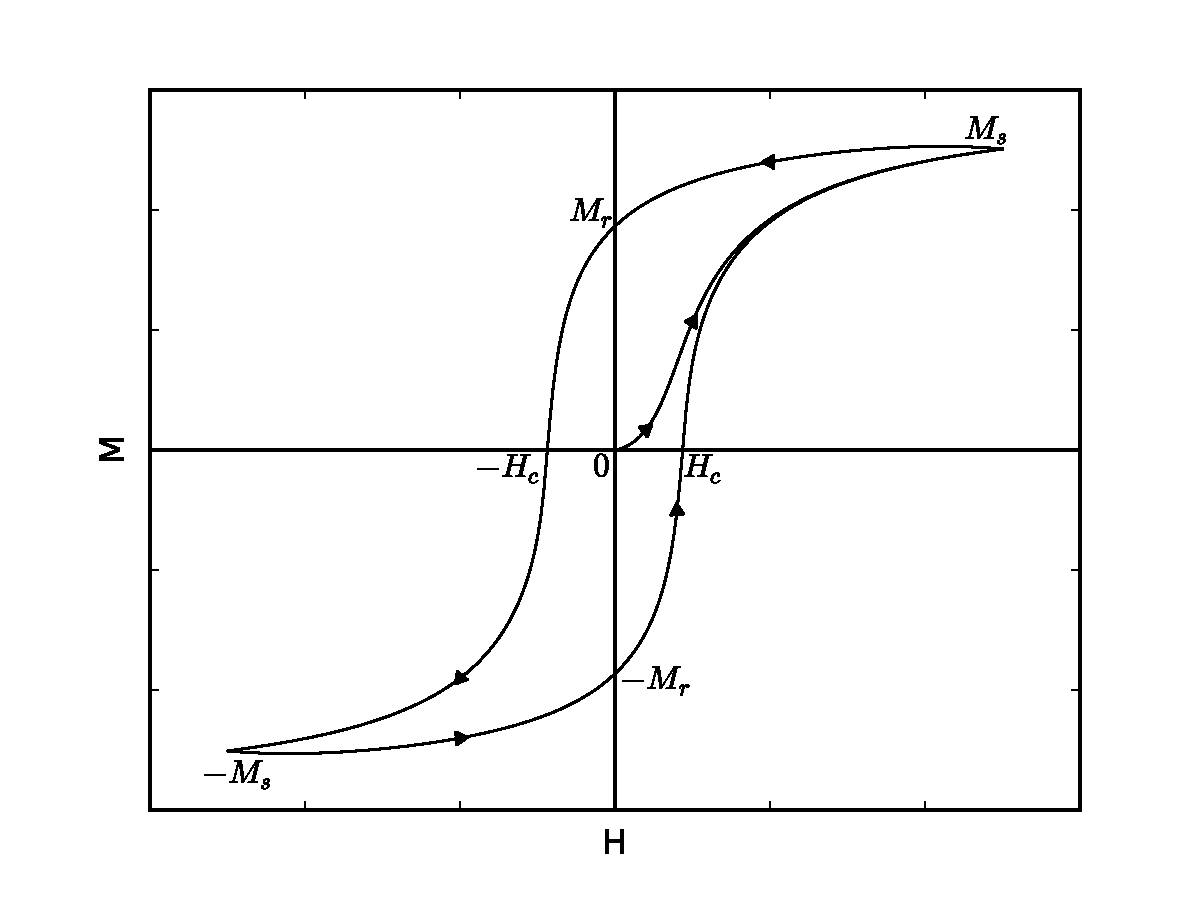
\includegraphics{figures/hysteresis_sample.pdf}}
\caption[Hysteresis loop of a ferromagnetic material]{Example of a hysteresis loop of a ferromagnetic material: $M_{r}$ is the remanent magnetization at H=0; ${H}_{c}$ is the coercivity, i.e. the reverse field that reduces $M$ to zero; $M_{s}$ is the saturation magnetization
\label{fig:hyst_loop}
}
\end{figure}

A typical hysteresis loop of a ferromagnetic material is shown in Figure \ref{fig:hyst_loop}. The upward curve starting at the origin is the inital magnetization curve which increases rapidly for increasing values of H until the saturation magnetization $M_{s}$ is reached. When H is now reduced, the magnetization decreases on a different curve. For a magnetic field intensity of zero the remanence magnetization $M_{r}$ is reached. In order to demagnetize the material a magnetic field, with a field intensity of $H_{c}$, also called the coercivity, must be applied in the opposite direction \cite{svoboda2004magnetic} \cite{sung2003physics} \cite{aharoni2000introduction}. \newline
Ferrimagnetic materials exhibit similar properties as ferromagentic materials as they both reach saturation and show much higher magnetization than either dia- or paramagnetic materials. As in ferromagnetic materials the magnetic moments are ordered regularly, but for ferrimagnetic materials in an antiparallel sense. However the opposing moments are unequal and a spontaneous magnetization still occurs. Ferrimagnetic behaviour is mainly shown by ferrites and mixed oxides of iron by example magnetite \cite{svoboda2004magnetic}\cite{michalowsky2006magnettechnik}.\newline
Ferro- and ferrimagnetic materials can also be divided by the value of their coercivity. Materials with a $H_{c}$ below 1\,kA/m are called magnetically soft, while materials with a larger value of $H_{c}$ are referred to as magnetically hard. Magnetically soft materials are easily magnetized, but exhibit only low remanent fields, in contrast magnetically hard materials will remain magnetized indefinitely unless they are demagnetized by an opposing magnetic field or heated above the Curie temperature \cite{meschede2015gerthsen}\cite{michalowsky2006magnettechnik}. 

\subsection{Influence of the particle shape and size}
\label{subsec:part_shape}


As already mentioned in Section \ref{subsec:Mag_mat}, the magnetic properties of ferromagnetic materials do not solely depend on the applied magnetic field, but also on the shape and size of the sample \cite{gomez2009influence}. The specific magnetic susceptibility $\chi$ is equivalent to $\kappa/\rho$, where $\kappa$ is the volume magnetic susceptibility and $\rho$ the material density. Therefore Equation \ref{eq:chi} can also be written as

\begin{equation}
\label{eq:kappa}
\centering
\boldsymbol{M} = \kappa\boldsymbol{H_{0}}
\end{equation}

Where an external, homogeneous magnetic field with a magnetic field intensity of $H_{0}$ is applied. Here $\kappa$ is not only dependent on the material, but also on the size and shape of the particle. The shape dependency can be explained by a demagnetizing field $H_{d}$ generated within the particle. The magnetic field $H_{i}$ inside the magnetized particle is not equal to the applied magnetic field $H_{0}$. The difference arises from the induction of a magnetic field $H_{d}$ inside of the finite ferromagnetic body of the particle opposing the external field. $H_{d}$ is proportional to $M$ as shown in Equation \ref{eq:demag_fac}. 

\begin{equation}
\label{eq:demag_fac}
\centering
\boldsymbol{H_{d}} = -N\boldsymbol{M}
\end{equation}

The dimensionless demagnetization factor $N$, with values in the range of 0 to 1, is dependent on the particle shape and the direction of magnetization. The inner magnetic field $H_{i}$ can therefore be calculated by Equation \ref{eq:int_field}. 

\begin{equation}
\label{eq:int_field}
\centering
\boldsymbol{H_{i}} = \boldsymbol{H_{0}} + \boldsymbol{H_{d}} = \boldsymbol{H_{0}} - N\boldsymbol{M}
\end{equation}

In case $N$ is known the magnetization of a material can be calculated solely from its material properties. 

\begin{equation}
\label{eq:mag_demag_fac}
\centering
\boldsymbol{M} = \frac{\kappa{i}}{1+N\kappa_{i}}\boldsymbol{H_{0}}
\end{equation}

Where $\kappa$ from Equation \ref{eq:kappa} is substituted by the fraction $\kappa_{i}/(1+N\kappa_{i})$ with the intrinsic susceptibility $\kappa_{i}$, which is the true susceptibility after the removal of the effects of $H_{d}$ \cite{FranzrebHabil}\cite{svoboda2004magnetic}.\newline 
The magnetic properties of ferromagentic materials are not only influenced by the shape, but also by the size of the particles. When the particle size is sufficiently small, the particle will consist of only a single magnetic domain (for further explanations of magnetic domains see Section \ref{subsec:Mag_mat}). Single domain nanoparticles have been experimentally observed, for example by Majetich and Jin \cite{majetich1999magnetization}. The maximum diameter for spherical single domain particles is called the critical size. The critical size lies e.g. at approximately 0.05\,\textmu m for magnetite \cite{svoboda2004magnetic}\cite{butler1975theoretical}. Single domain particles are considered to be magnetized to saturation in one or the opposite direction, even if no external field is applied. Due to thermal motion the magnetization will fluctuate randomly between the two directions. This behaviour is called superparamagnetism.
Superparamagnetism is based on the same mechanism as paramagnetism, except that the magnetic moments are replaced by the moments of the entire particle. Measurements of the magnetization of a larger number of superparamagnetic particles result in an observed net magnetization of zero, as the magnetization of each particle is oriented randomly. When an external field is applied, the moments of the particles will align and the net magnetization increases until saturation is reached. Once the field is removed, however, the particle moments will lose coherence and no net magnetization is retained. Consequently superparamagnetic particles show a coercivity and remanence of zero similar to paramagnetic materials combined with a high saturation magnetization comparable to ferromagnetic matter \cite{svoboda2004magnetic}\cite{FranzrebHabil}.      
    
\section{Fundamentals of magnetic separation}
\label{sec:Mag_sep}
\textbf{Markus: mir wurde jetzt gesagt, dass ich die verschiedenen Theorieteil in meine Arbeit einordnen soll mit nem Satz; hier z.B: magnetic seperators are used in this study for ... see Section}
Since the 19\textsuperscript{th} century magnetic separation processes have been used to concentrate and separate minerals. More recently, applications in waste water treatment, food industry and biotechnology have become available \cite{yavuz2009magnetic}. Magnetic separation technologies are used for the concentration of magnetic materials  as well as the removal of magnetizable particles from process fluids. As this work concentrates mainly on the use of magnetic separation for solid-liquide separation, the following sections will only describe the separation of magnetizable particles from suspensions. For separation \textbf{Markus: separation between what, das hast du noch nicht beschrieben} the magnetic particles within a suspension are influenced by a non-homogeneous magnetic field, which leads to either retention or deflection of the particles. The external magnetic field can be generated by a permanent magnet or an electromagnet. In addition, the particles are influenced by other external forces e.g. gravitational, inertial, hydrodynamic and centrifugal forces. Furthermore electrostatic and electromagnetic interparticle forces affect the separation. Consequently, the magnetic force $F_{mag}$ must be greater than the sum of the competing forces $F_{comp}$ \textbf{Markus: evtl Referenz dorthin wo du die verschiedenen Fcomp aufzählst}  for successful separation of the particles from the surrounding fluid. For a selective separation of particles with different magnetic susceptibilities, the magnetic force acting on the more magnetic \textbf{Markus: ist "more magnetic" wirklich wissenschaftlich} particles must be larger than the sum of $F_{comp}$ and for less magnetic particles smaller than the sum of $F_{comp}$. This condition is described in Equation \ref{eq:mag_sep_cond}, where $F_{mag}^{m}$ and $F_{mag}^{n}$ are the magnetic forces affecting the more and less strongly magnetic materials respectively and $F_{comp}$ summarizes the competing forces on the different particles \cite{svoboda2004magnetic}\cite{oberteuffer1974magnetic}.   \textbf{Markus: warum haben die "less magnetic" particle then index n statt l (wegen non-magnetic?)}

\begin{equation}
\label{eq:mag_sep_cond}
\centering
F_{mag}^{m}\geq\sum_{i}F_{comp}^{im} \quad \textrm{and} \quad F_{mag}^{n}\leq\sum_{i}F_{comp}^{in}
\end{equation}
\textbf{Markus: hier kannst du einen Übergang zu dem ersten Unterkapitel oder sogar ein einordnen der ganzen Unterkapitel machen, dass der Leser weiß warum du das so machst}
\subsection{Basic principles}
\label{subsec:bas_princ}
The concept of magnetic separation is based on the property of magnetic fields to exert a force on matter. The magnetic force $F_{m}$ on a particle is given by \textbf{Markus: : (Doppelpunkt einfügen?)}

\begin{equation}
\label{eq:mag_force}
\centering
\boldsymbol{F}_{m} = \mu_{0}V_{p}\boldsymbol{M}_{p}\nabla\boldsymbol{H}
\end{equation}

\textbf{Markus: ,}where $V_{p}$ denotes the volume of the particle, $\boldsymbol{M}_{p}$ the particle magnetization and $\nabla\boldsymbol{H}$ the gradient of the applied magnetic field. For reasons of simplification $F_{m}$ is assumed to act on the center of gravity of the particle. $\boldsymbol{M}_{p}$ can be calculated by either \textbf{Markus: oder either by} Equation \ref{eq:chi}, \ref{eq:kappa} or \ref{eq:mag_demag_fac}. As shown in Table \ref{table:mag_material}, the magnetic susceptibility for diamagnetic and paramagnetic materials is constant, while $\chi$ for ferromagnetic and ferrimagnetic substances is dependent on the magnetic field strength, the size and the shape of the particles (see Sections \ref{subsec:Mag_mat} and \ref{subsec:part_shape}). For spherical particles $F_{m}$ is also directly proportional to the cube of the particle radius $b$ \textbf{Markus $b^3$ liest sich einfacher}. \newline
As already mentioned above (see Section \ref{sec:Mag_sep}), the motion of the particles is also influenced by several different  forces. For ferromagnetic particles larger than approximately 1\,\textmu m the relevant competing forces are  the hydrodynamic drag force $F_{d}$, to a lesser degree in liquids the gravitational force $F_{g}$ and depending on the separator type the centrifugal force $F_{c}$.  


\begin{equation}
\label{eq:grav_force}
\centering
\boldsymbol{F}_{g} = (\rho_{p}-\rho_{f})V_{p}\boldsymbol{g}
\end{equation}

\begin{equation}
\label{eq:drag_force}
\centering
\boldsymbol{F}_{d} = 6\pi\eta b(\boldsymbol{v}_{f}-\boldsymbol{v}_{p})
\end{equation}

\begin{equation}
\label{eq:cent_force}
\centering
\boldsymbol{F}_{c} = (\boldsymbol{v}_{f}-\boldsymbol{v}_{p})\omega V_{p}\boldsymbol{r}
\end{equation}

$F_{g}$ for a spherical particle is given by Equation \ref{eq:grav_force}, where $g$ is the acceleration by gravity and $\rho_{p}$ and $\rho_{f}$ are the densities of the particle and the surrounding fluid, respectively. The hydrodynamic drag force of a particle is determined by Stoke's law \textbf{markus: gilt das nicht nur für einen bestimmten Bereich der Rayleigh Zahl? also bei riesigen Geschwindigkeiten nicht mehr gelten, wenn z.B. deine Säule gerade explodiert;-)} (see Equation \ref{eq:drag_force}), where $\eta$ denotes the dynamic viscosity of the fluid, $v_{f}$ the velocity of the fluid and $v_{p}$ the velocity of the particle. $F_{c}$ is described by Equation \ref{eq:cent_force}, where $\omega$ is the angular velocity and $r$ is the radial position of the particle. Equation \ref{eq:force_rad} shows the dependency of the different forces on the particle radius $b$ \textbf{Markus: which is already obvious in Equation \ref{eq:grav_force} to \ref{eq:cent_force}} . 

\begin{equation}
\label{eq:force_rad}
\centering
F_{g}\sim b^{3}, \quad F_{d}\sim b^{1} \quad \textrm{and} \quad F_{c}\sim b^{3}
\end{equation}

$F_{g}$ and $F_{c}$ are directly proportional to the cube of the particle radius, consequently their contribution increases significantly with increasing particle size. $F_{d}$ however depends on the first power of the particle radius and will be relevant for smaller particles \cite{svoboda2004magnetic}\cite{oberteuffer1974magnetic}. For particles smaller than approximately 1\,\textmu m Brownian motion also needs to be considered. Brownian motion is the apparently random movement of particles in a fluid due to their collisions with other \textbf{Markus: other particles,} atoms or molecules of the fluid \cite{brown1828xxvii}. Brownian motion can be described by the   
Langevin equation (for more detailed information see \cite{Langevin}\cite{BrownianDynamics} \cite{BrownianModel}). It states that the minute fluctuations in the position of the particles are due to a random force. Einstein and Sutherland obtained a relation between the macroscopic diffusion constant $D$ and the atomic properties of matter \cite{einstein1906theorie}\cite{einstein1905molekularkinetischen}\cite{sutherland1905lxxv}. 

\begin{equation}
\label{eq:Stokes_Einstein}
\centering
D = \frac{k_{B}T}{6\pi\eta b}
\end{equation}

Equation \ref{eq:Stokes_Einstein}, called Stokes-Einstein equation, describes the diffusion of spherical particles through a fluid with low Reynolds numbers. $k_{B}$ is the Boltzmann constant with a value of 1.38064852$\cdotp$10\textsuperscript{-23}\,J/K \textbf{markus: das ist aber genau angegeben, ich hoffe du kannst bei deinem Vortrag auf nachfrage auch die 8te Nachkommastelle nennen;-)}, which can be calculated by the division of the universal gas constant $R$ by the Avogadro constant $N_{A}$, while T \textbf{Markus: ist ne variable also kursiv} is the temperature of the surrounding fluid. Particle diffusion can be pictured as a driving force which is based on the gradient in the particle concentration. 
A "diffusion force" $F_{B}$ acting on the particles can therefore be described as follows:

\begin{equation}
\label{eq:mag_force}
\centering
\boldsymbol{F}_{B} = -k_{B}T\frac{\nabla n}{n}
\end{equation}

\textbf{Markus: ok du machst hier wohl absichtlich kein Komma}where $n$ is the number density of particles within the fluid \cite{choomphon2017simulation}\cite{moeser2004high}\cite{fletcher1991fine}. \\
As the type of particles (\textbf{Markus: described by its} shape, size, material) is usually given, the main influencing factors on $F_{m}$ for the magnetic separation are the magnetic field strength and its gradient. Consequently the combination of magnetic field strength and field gradient must be optimized for each application individually. The most common magnetic separators can be divided into three basic categories: open gradient magnetic seperators, closed-gradient magnetic separators and matrix (polygradient) magnetic seperators \cite{svoboda2004magnetic}. \Gls{hgms} \textbf{Markus: hast du das schon irgendwo eingeführt?}, which are used for the recovery of micron sized particles, belong to the class of matrix separators. In the following Section \textbf{Markus: section klein wenn keine Zahl dahintersteht} the principles of \gls{hgms} will be further explained.  


\subsection{High gradient magnetic separation}
\label{subsec:HGMS}
In conventional magnetic separators only ferromagnetic materials with a particle size larger than approximately 50\,\textmu m can be separated. \Gls{hgms}, based on the Frantz Ferrofilter, enables the magnetic separation of smaller and only weakly magnetic particles \cite{frantz1937patent} \cite{ge2017magnetic}. This is achieved through the combination of strong magnetic fields and high magnetic field gradients. Ferromagnetic bodies, called the matrix, are placed in the external magnetic field. The applied magnetic field induces magnetic moments in the ferromagnetic matrix which leads to high magnetic field gradients in the proximity of the matrix elements \cite{shukla2006process}. Magnetically susceptible particles will move \textbf{markus: will move oder nur move? genauso bei will be captured/are captured} along the gradient towards the magnetized matrix elements and will be captured on the surface \cite{hoffmann2002novel}. As the magnitude of the magnetic field gradient as well as the collection surface are dependant on the shape, size, arrangement and placement of the used bodies, the matrix material e.g. balls, grooved plates, steel wool or rods has to be chosen carefully (more information on different matrix materials can be found in \cite{iacob2002high}\cite{kim2013effects}\cite{takayasu1981matrices}). The matrix has to be fine enough to generate a strong enough magnetic field gradient for selective separation, but also not so strong as to cause matrix blockage and retention of non-magnetic materials. As the filling factor of the used matrix material is often low, e.g. 0.04 and 0.20 for steel wool and expanded metal respectively and as the matrix does not conduct magnetic flux very well, strong external fields are required. An exception are matrices consisting of balls with a filling factor of up to 0.50 and grooved plates with a filling factor of 0.80. 
%In general, the separation efficiency of ball matrices is smaller than the in filament units, as a closed packed array of spheres does not leave much space for the collection of particles.  


%%%%%%%%%%%%Include Figure of HGMS%%%%%%%%%%%%%%%%%%%%%%%%%%%%%%%%%%%%%%%%%%%%%%%%%%%%%%change figure !!!!!!!!!!!!!!!!!

\begin{figure}[h]
\centering

\scalebox{0.35}{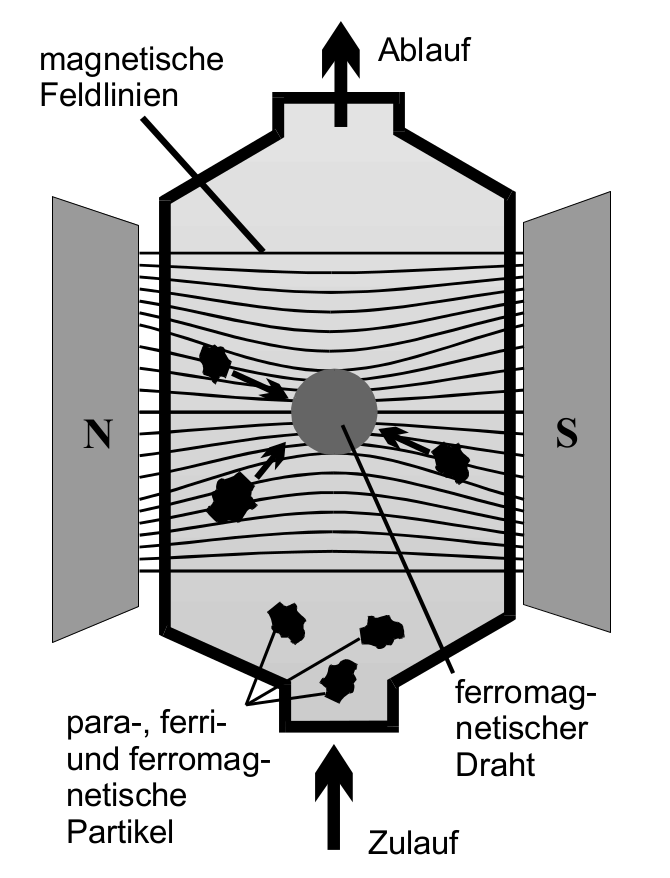
\includegraphics{figures/hgms_franzreb.png}}
\caption[Schematic \gls{hgms} process]{Schematic \gls{hgms} process: The ferromagnetic wire placed in the external field, generated by permanent magnets, generates high magnetic field gradients. The magnetic particles in the suspension move along the gradient towards the wire and are captured on the wire's surface \cite{FranzrebHabil}.  
\label{fig:hgms}
}
\end{figure}

A schematic drawing of a \gls{hgms} is shown in Figure \ref{fig:hgms}. The particle suspension flows through the matrix. Particles with high magnetic susceptibilities accumulate on the matrix surface while the rest of the suspension leaves the system. Once the matrix is saturated with particles, the external magnetic field is turned off and the collected particles are recovered \cite{svoboda2004magnetic}\cite{gerber1983high}\cite{ditsch2005high}.    
\textbf{Markus: hier könnte auch eine Überleitung hin}
\subsection{Magnetic field in the vicinity of a magnetized wire}
\label{subsec:mag_field}
The magnetic field $H(r,\varphi)$ in the vicinity of a infinitely long cylinder, which is magnetized by a homogeneous magnetic field $H_{0}$ (configuration shown in Figure \ref{fig:wire}), is described by the following equation: \textbf{Markus: du musst evtl formal noch phi und r einführen, z.B Mittelpunkt deines Koordinatensystems, auch wenn das eigentlich offensichtlich ist}

\begin{equation}
\label{eq:mag_field_strat}
\centering
H = H_{0}(e_{r}cos\varphi-e_{\varphi}sin\varphi)+H_{0}\frac{a^{2}}{r^{2}}\left(\frac{\mu_{w}-\mu_{f}}{\mu_{w}+\mu_{f}}\right)(e_{r}cos\varphi+e_{\varphi}sin\varphi)
\end{equation}

where $e_{r}$ and $e_{\varphi}$ are the unit vectors in the polar coordinate system and $\mu_{w}$ and $\mu_{f}$ depict the magnetic permeability of the wire and the fluid, respectively \cite{stratton2007electromagnetic}. For an external field $H_{0}$, that is strong enough to magnetize the wire to saturation, and a surrounding medium with a permeability close to one, e.g. water or air, Equation \ref{eq:mag_field_strat} can be written as follows:

\begin{equation}
\label{eq:Hr_field}
\centering
H_{r} = \left(\frac{M_{s,w}a^{2}}{2r^{2}}+H_{0}\right)cos\varphi
\end{equation}
%%%%%%%%%%%%%%%%sin\theta ???cos\theta????????%%%%%%%%%%%%%%%%%%%%%%%%%%%%%%%%%%%%
\begin{equation}
\label{eq:Hphi_field}
\centering
H_{\varphi} = \left(\frac{M_{s,w}a^{2}}{2r^{2}}-H_{0}\right)sin\varphi
\end{equation}

where $a$ is the radius of the wire and $r$ is the distance between the wire and the magnetic nanoparticle \cite{FranzrebHabil}. The magnetic field of a magnetized ferromagentic wire is shown in Figure \ref{fig:mag_field_wire}. The magnetic force $F_{m}$ affecting the particles can then be calculated from the magnetic field with Equation \ref{eq:mag_force} \cite{moeser2004high}. 

\begin{figure}[H]
\centering
\scalebox{0.4}{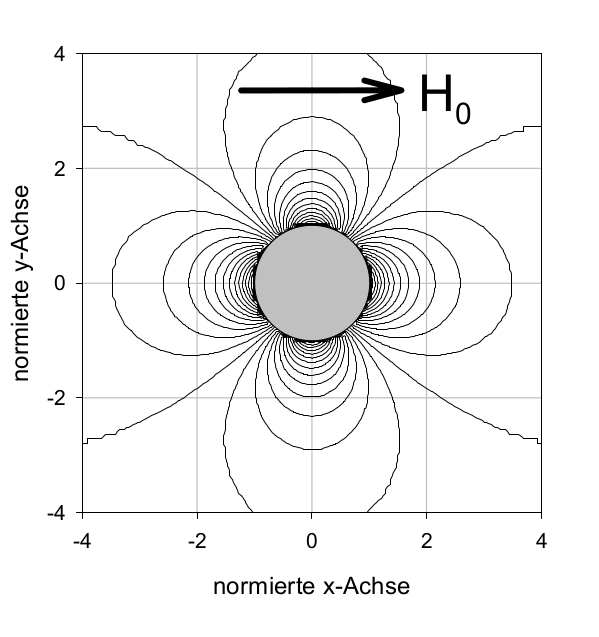
\includegraphics{figures/mag_field_wire_franz.png}}
\caption[Magnetic field in the vicinity of a wire]{Field lines of a magnetic field in the vicinity of a magnetized ferromagnetic wire\cite{FranzrebHabil} \textbf{markus: die achsen sind halt deutsch: mach sie englisch und sag (modified) ;-)}
\label{fig:mag_field_wire}
}
\end{figure}

\subsection{Magnetic particle accumulation on single wires}
\label{subsec:single_wire}
For micron-size particles or larger, the \gls{hgms} collection process can be simplified by the analysis of a single magnetized collector and the particle trajectories in its vicinity. Figure \ref{fig:wire} depicts the configuration of particle capture in a single wire model.

\begin{figure}[h]
\centering
\scalebox{0.3}{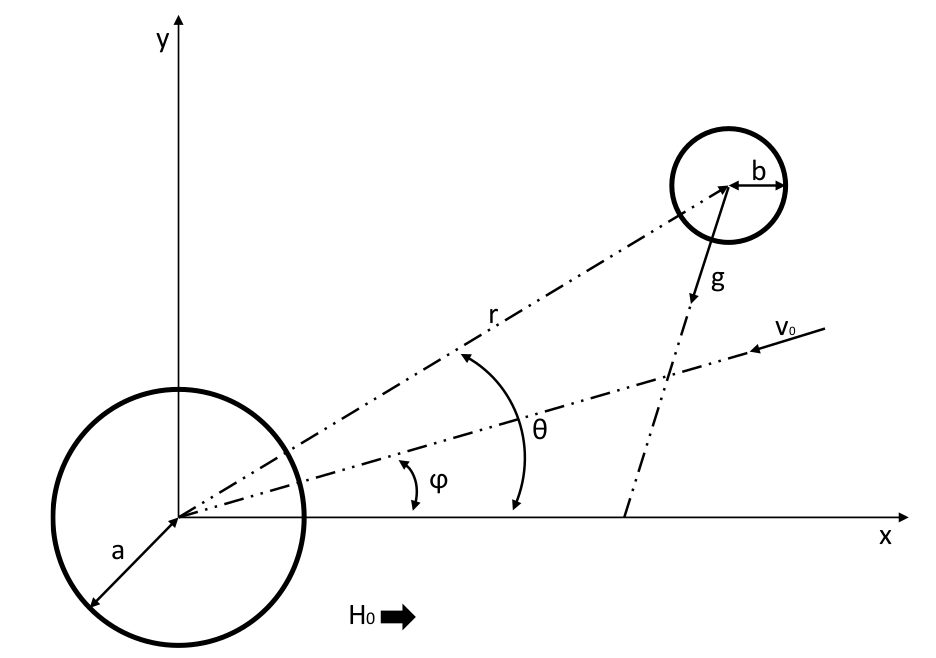
\includegraphics{figures/Single_wire.png}}
\caption[Configuration of particle capture in a single wire model]{Configuration of particle capture in a single wire model: A cylindrical ferromagnetic wire with the radius $a$, which is magnetized to saturation by an external magnetic field $H_{0}$, a paramagnetic particle with the radius $b$ at a distance $r$ from the wire and a polar angle of $\theta$ from the wire center and the fluid flow velocity $v_{0}$ \cite{svoboda2004magnetic}
\label{fig:wire}
}
\end{figure}

For a single wire model three different orientations of the wire relative to the flow and applied field are considered. It is assumed that the magnetic field is always orthogonal to the ferromagnetic wire. The direction of the fluid flow can then be either parallel (longitudinal) or perpendicular (transversal) to the direction of the magnetic field. In addition, the fluid flow can be oriented parallel to the wire, which is referred to as axial configuration \cite{friedlaender1978particle}. The particle build-up profiles for the three different orientations are shown in Figure \ref{fig:hgms_config}.   

\begin{figure}[h]
\centering

\scalebox{0.45}{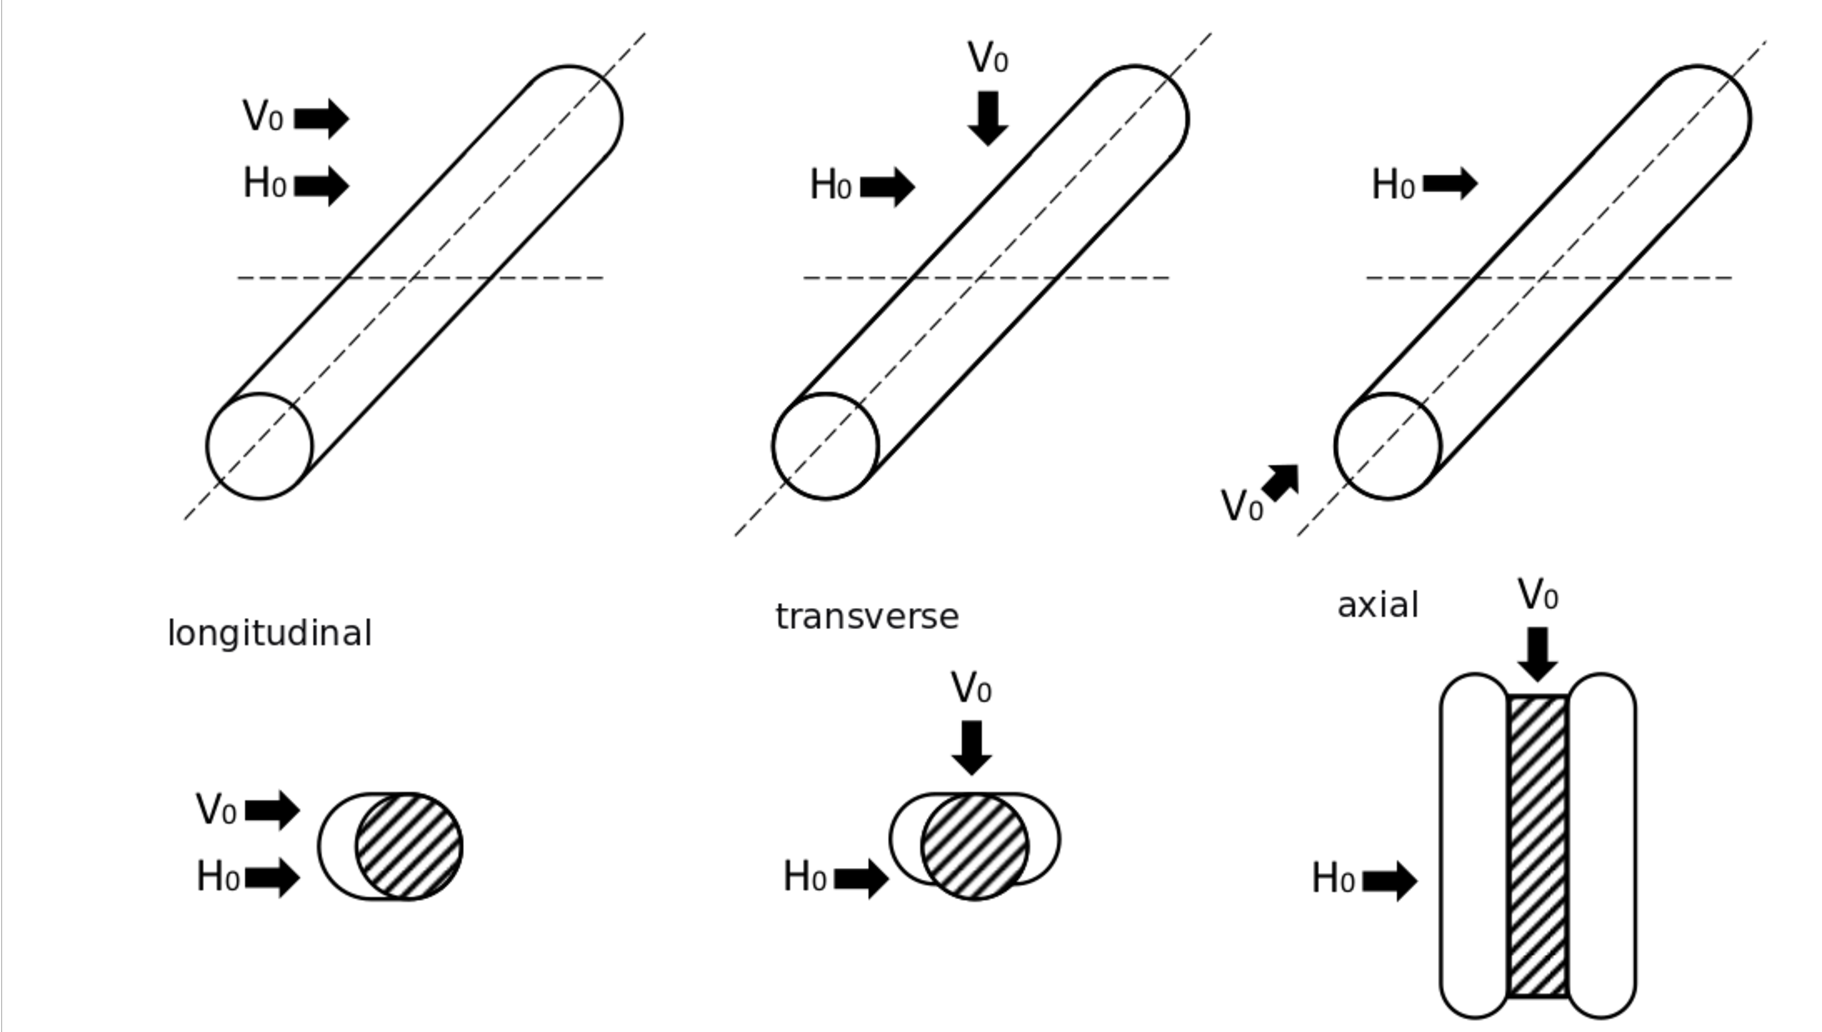
\includegraphics{figures/hgms_orientation.pdf}}
\caption[Geometric configurations in \gls{hgms} and particle build-up]{Schematic drawing of the three main geometric configurations in \gls{hgms} and the corresponding profiles of the particle build-up in a ferromagnetic wire; arrangements between the directions of the magnetic field $H_{0}$ and the particle flow velocity $v_{0}$ with respect to the wire (top) and the cross section of the wire (hatched area) with the particle build-up profile corresponding to the respective configuration \cite{svoboda2004magnetic}
\label{fig:hgms_config}
}
\end{figure}

The particle trajectories in the vicinity of the wire are calculated by Newton's second law, which states that the sum of all forces affecting the particle is equal to the product of the particle mass $m$ and its acceleration $a_{p}$. 

\begin{equation}
\label{eq:mag_force}
\centering
\sum_{i}\boldsymbol{F}_{i} = m\boldsymbol{a}_{p}
\end{equation}
 
The forces acting on the particles e.g. the magnetic, gravitational and hydrodynamic force are described in Section \ref{subsec:bas_princ}. Whether a particle is collected by the wire or not can be determined by following the particle trajectory. If the particle trajectory ends on the wire's surface, the particle is separated, if, however, the particle trajectory passes the wire the particle remains in suspension \cite{FranzrebHabil}. A model for particle trajectories with a sphere instead of a wire can be found in \cite{friedlaender1981particle}\cite{moyer1986filtration}. \newline 
In the case of ultra-fine magnetic particles, where the diffusion outweighs the other forces, the trajectory analysis is not suitable. In this case, the continuity equation representing the conservation of mass with the influence of external forces on individual magnetic particles expressed through the flux term is solved \cite{choomphon2017simulation}. In a two-dimensional model spherical and cylindrical collectors are treated in the same way. The solution of the continuity equation, describing the time-dependent distribution of the magentic particles around the collector, can be written as follows:     

\begin{equation}
\label{eq:diff_eq}
\centering
\frac{\partial n}{\partial t} = \nabla\cdotp(D\nabla n)-\nabla\cdotp(n v_{p})
\end{equation}

where $n$ is the particle number density, $D$ the diffusion coefficient and $v_{p}$ the particle drift velocity caused by the magnetic force $F_{m}$ for spherical particles at low Reynolds numbers. $D$ is determined by the Stokes-Einstein relation (see Section \ref{subsec:bas_princ}). For a steady-state, i.e. ${\partial n}/{\partial t}$=0, Equation \ref{eq:diff_eq} reduces to:

\begin{equation}
\label{eq:diff_eq}
\centering
 D\nabla n = n v_{p}
\end{equation}

which describes the dynamic balance between an inward flux of the particles towards the wire and an outward flux due to Brownian motion \cite{fletcher1991fine}. 



% Diffusion with force balance: \cite{gerber1983generalization}\cite{takayasu1983magnetic}\cite{davies19902}\cite{fletcher1991fine}
% Diffusion with energy model \cite{glew1984influence}
% 
%  \cite{choomphon2017simulation}
% \cite{moyer1986filtration} for spheres as matrix


% \section{Dimensioning of a Helmholtz coil}
% \label{sec:Dim_helm_coil}
% A Helmholtz coil produces an approximately uniform magnetic field along the x-axis between the coils. The dimensioning of the coil is based on the Biot-Savart law, which describes the magentic field generated by a stationary electric current. The magnetic flux density in a cylindrical coil with only one winding can be calculated with Equation \ref{eq:one_winding}. 
% 
% \begin{equation}
% \label{eq:one_winding}
% \centering
%  B(r) = \frac{\mu_{0}}{4\pi}\int d^{3}r^{'}j(r^{'}\times \frac{r-r^{'}}{\vert r-r^{'} \vert^{3}}
% \end{equation}
% 
% Where $d^{3}r^{'}$ denotes a volume integral, $j(r^{'}$ the current density and $r-r^{'}$ a direction vector. In addition the vectors $r$ and $r^{'}$ are defined as the following: $r = (0,0,z)$ and $r^{'} = (R cos(\phi),R sin(\phi), z^{'})$. 
% 
% \cite{wotruba1968verbesserung}\cite{wotruba1969massive}\cite{heller1955erzeugung}
%%%%%%%%%%%%%%%%%really necessary??%%%%%%%%%%%%%%%%%%%%%%%%%%%%%%%%%%%%%%%%

\section{Computational fluid dynamics}
\label{sec:CFD}
\Gls{cfd} is an well established method in fluid mechanics. It enables a quick and efficient analysis of fluid flow, heat transfer and related phenomena through computer-based numerical analysis \cite{versteeg2007introduction}. Formerly mainly used for numerical weather prediction, calculations concerning the aerodynamics of airplanes and power generation, it has now become a vital component in process and
product development in many different aspects of engineering. Applications now
vary from chemical process and civil engineering to biomedical and pharmaceutical
process and product design. CFD offers an inexpensive alternative to experimental approaches as well as the possibility to study systems in which experiments
would be unfeasible. Other main advantages include the reduced time, parallel processing and the almost unlimited level of detail of results. The progress in both hardware and numerical algorithms in the past decades has led to the development of numerous commercial and open-source CFD programs \cite{ghia1982high}. In this work a numerical model using the COMSOL Multiphysics software was developed.

\subsection{Navier-Stokes equations}
\label{subsec:Navier_Stokes}
The Navier-Stokes equations are a macroscopic model of the motion of viscous fluids. There are only analytical solutions for simplified forms of the Navier-Stokes equations e.g. Couette flow and Hagen-Poiseuille flow. For more complex, nonlinear problems the equations need to be solved numerically. The Navier-Stokes equations for a incompressible Newtonian fluid can be written as follows: 

\begin{equation}
{\partial{\bf u}\over{\partial t}} + ({\bf u} \cdot \nabla) {\bf u} - \nu\Delta{\bf u}+ \nabla p = {\bf F}
\label{eq:Concervation of momentum }
\end{equation}

\begin{equation}
\nabla{\bf u} = 0
\label{eq:Conservation of mass }
\end{equation}

where $u$ is the fluid velocity, $p$ is the fluid pressure, $\nu$ is the kinematic viscosity and $F$ is the sum of all external forces \cite{versteeg2007introduction}. The first term describes the local acceleration of the fluid, ${\bf u} \cdot \nabla) {\bf u}$ is the non-linear convective term describing the inertial forces, $\nabla p$ is the pressure gradient and $\nu\Delta{\bf u}$ is called the dissipative viscous term. The Navier-Stokes equations are always solved together with the continuity equation (see Equation \ref{eq:Conservation of mass }). The Navier-Stokes equations satisfy the conservation of momentum, while mass conservation is included through the continuity equation \cite{alkahtani2013numerical}. The Reynolds number is a dimensionless quantity in fluid dynamics, which is used to characterize a fluid flow. The Reynolds number is defined as the ratio of the inertial forces to the viscous forces and can be written as:  

\begin{equation}
Re=\frac{\rho u L}{\mu}=\frac{uL}{\nu}
\label{eq:Reynolds}
\end{equation}

where $\rho$ is the fluid density in kg/m\textsuperscript{3}, $L$ is a characteristic linear dimension in m, e.g. the hydraulic diameter of a pipe, and the dynamic viscosity $\mu$ of the fluid in Pa$\cdotp$s. For a low Reynolds number the flow condition will be laminar, while for higher Reynolds numbers, over approximately 2300 for flow in a circular pipe, turbulent flow occurs \cite{schwarze2012cfd}. Flows where Re$\ll$1 are referred to as Stokes flow or creeping flow. Here the viscous forces are much larger than the inertial forces which is usually achieved by either very low velocities or small characteristic lengths. Stokes flow also occurs in highly viscous fluids such as heavy oils and honey \cite{lautrup2004physics}. Figure \ref{fig:creep_tot} shows creeping flow around a cylinder as a schematic drawing and in reality. 

\begin{figure}[H]
		%\centering
          \begin{subfigure}{0.49\textwidth}
                  \flushleft
                  \scalebox{0.13}{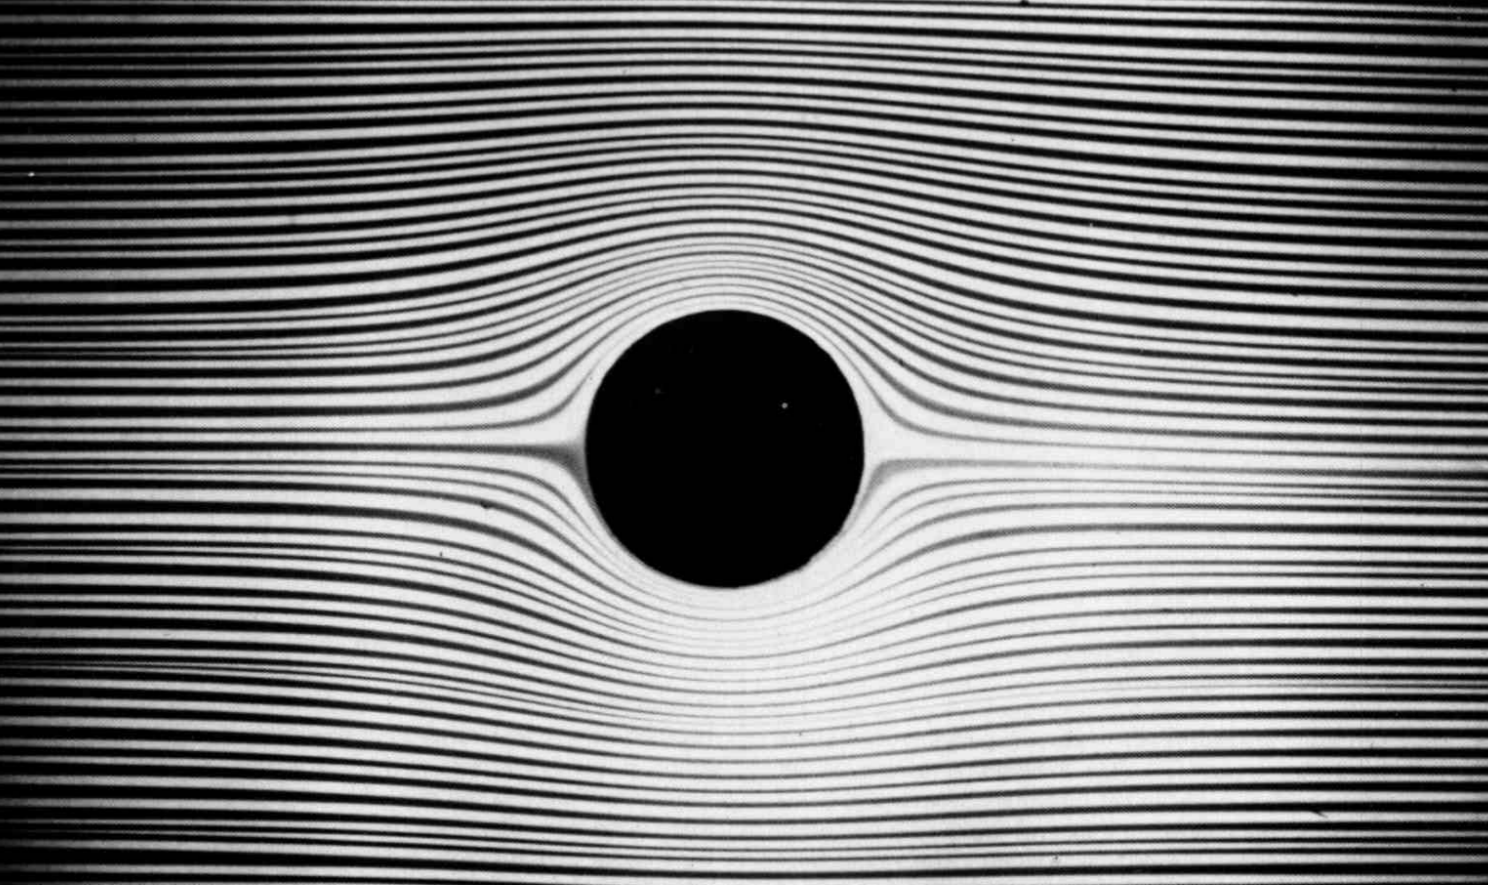
\includegraphics{figures/Creeping_flow_around_Cylinder.png}}
                  \caption{Streamlines in water flowing past a cylinder with a velocity of 1\,mm/s between glass plates placed 1\,mm apart visualized with dye \cite{van1982album}\label{fig:creep_1}}
          \end{subfigure}\hfill
        \begin{subfigure}{0.49\textwidth}
                \flushright
                \scalebox{0.358}{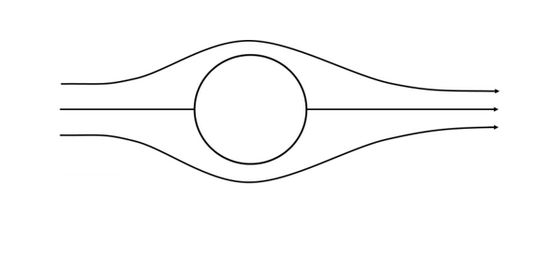
\includegraphics{figures/Creeping_flow_around_cylinder_schematic_4.png}}
                \caption{Schematic drawing of the streamlines around a cylinder for creeping flow}\label{fig:creep_2}
        \end{subfigure}
        \\
        
        \caption[Creeping flow around a cylinder]{Flow field for a creeping flow around a cylinder with Re$\ll$1 }
        \label{fig:creep_tot}
  \end{figure}

\subsection{Space and time discretization methods}
\label{subsec:FEM}
Space and time dependent physical problems are usually described with the help of \gls{pde} in a domain $\Omega$. Most of these \gls{pde} cannot be solved with analytical methods, but an approximation of the equations based on different types of discretizations can be obtained. \Gls{fem} is a numerical technique for constructing such approximate solutions for \gls{pde}. The principle of the method is to replace an entire continuous domain by a number of finite-sized subdomains, called elements, of geometrically simple shapes like tetrahedrons or triangular prism. Together the elements constitute the finite-element mesh. The \gls{pde} for each element are approximated by an interpolation function, such as a linear, quadratic or higher order polynomial, also referred to as basis function, with a finite number of degrees of freedom. In combination with the boundary conditions a  system of algebraic equations is obtained, which can be solved by a sparse matrix solver \cite{john2016finite}. The solution of the matrix results in an approximate solution of the \gls{pde}. The accuracy of the solution can be increased by a refinement of the finite-element mesh or an increased order of the basis function. An example of the approximation of a function $u$ by the function $u_{h}$ consisting of linear combinations of basis functions $\psi_{i}$ with the coefficients $u_{i}$ (see Equation \ref{eq:FEM}) is depicted in Figure \ref{fig:FEM}. 

\begin{equation}
u\approx u_{h} \quad \textrm{with} \quad u_{h}=\sum_{i}u_{i}\psi_{i}
\label{eq:FEM}
\end{equation}

\begin{figure}[H]
\centering
\scalebox{0.3}{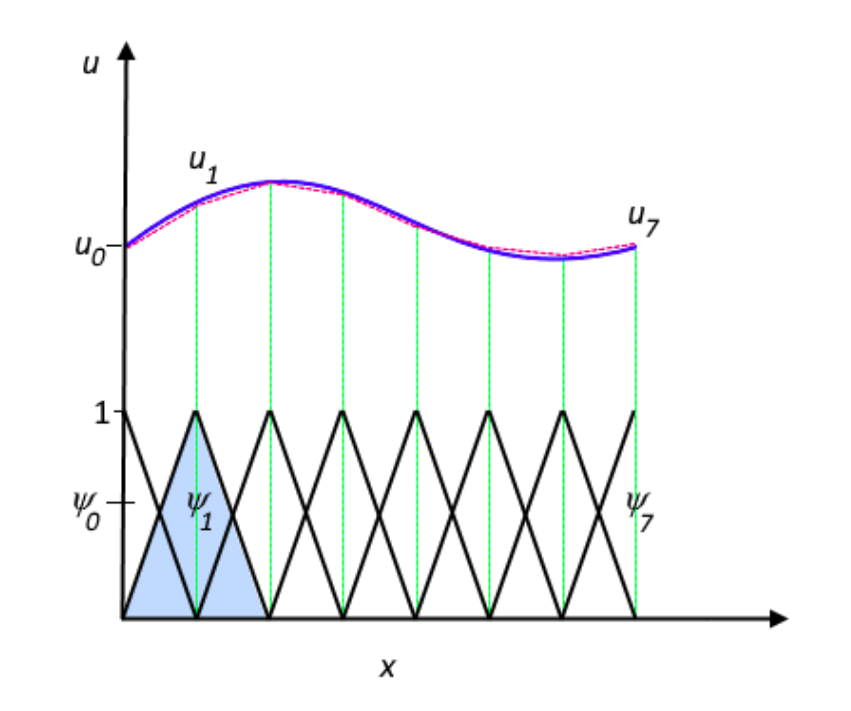
\includegraphics{figures/FEM.png}}
\caption[]{Approximation of the function $u$ (solid blue line) with the function $u_{h}$ (dashed red line), where $u_{h}$ is a combination of linear interpolation functions $\psi_{i}$ (solid black lines) and the coefficients $u_{0}$ to $u_{7}$ \cite{ComsolFEM}
\label{fig:FEM}
}
\end{figure}

Overall \gls{fem} for the approximation of \gls{pde} can be divided into four steps: Discretization of the domain, selection of the interpolation functions, formulation of the system equations and solution of the system equations. \newline 
\Gls{fem} can also be applied for a time domain, this can however be coupled with a high computational effort. Therefore simple time-stepping methods based on finite differences are frequently used for time discretization. The implicit time-stepping algoritm used in this work is the \gls{bdf} solver, which uses backward differentiation formulas with the order of accuracy varying from one, known as the backward Euler method, to five. \Gls{bdf} solvers exhibit a high their stability, but also includes more damping effects than comparable solvers based on e.g. generalized alpha or Runge-Kutta methods \cite{ComsolRefManual}.  

\section{Simulated moving bed chromatography}
\label{sec:smb}
\gls{smb} was developed in the late 1950s by engineers from Unviersal Oil Products to seperate p-xylene from its isomers \cite{broughton1961continuous} \cite{carson1962rotary}. The invention the continuous process was mainly motivated by the need to produce large quantities of chemicals at high purity. 


\chapter{Materials and Methodology}
\label{chap:chap_mat}
\newacronym{pva}{PVA}{polyvinyl alcohol}
\newacronym{pmma}{PMMA}{polymethyl methacrylate}
\newacronym{ptfe}{PTFE}{polytetrafluorethylen}
\newacronym{fplc}{FPLC}{Fast Protein Liquide Chromatography}
\newacronym{esem}{ESEM}{Environmental scanning electron microscope}
\newacronym{agm}{AGM}{Alternating Gradient Magnetometer}

In the first part of this chapter the model setup and implementation using the simulation software COMSOL Multiphysics\textsuperscript{\textregistered}, thereafter referred to as COMSOL, is described.\\
Section \ref{sec:Exp_setup} gives an overview of the experimental setup and execution as well as the analytical and evaluation methods used.  


\section{Model setup/Development}
\label{sec:Model_setup}
The objective of this thesis was the design and implementation of (to establish) an in silico model simulating the retention of magnetic nanoparticles flowing through a magnetizable packed bed. Furthermore parameter studies for various conditions were conducted. In the following the simulation setup including geometry, mesh, boundary conditions and solvers is described.    


\subsection{Model validation/verification}
\label{subsec:model_val}
Benchmark problem flow around a cylinder (Schaefer and Turek)
Comparison of drag coefficients

Comparison with analytical solution of magnetic field around a wire

\section{Experimental setup}
\label{sec:Exp_setup}
For the validation of the simulation results and a proof of principle of the operational concept several experimental runs were designed. In order to evaluate the retention of a magnetic nanoparticle suspension within a magnetizable packed bed a chromatographic system was used (see Section \ref{subsec:chrom_sys}). The nanoparticle suspension is characterized in Section \ref{subsec:Mag_nanoparticles} and the matrix materials in Section \ref{subsec:Matrix_mat}. Furthermore an overview of the conducted experiments is given in Section \ref{subsec:Exp_Pro}. In Section \ref{subsec:ana_met} the analytical methods and in Section \ref{subsec:Eval} the evaluation methods are discussed.    


\subsection{Magnetic nanoparticle suspension}
\label{subsec:Mag_nanoparticles}
The experiments were conducted with two different types of magnetic nanoparticles. For the experiments in Section \ref{subsec:Exp_Pro} a nanoparticle suspension from Chemagen (Chemagen Biopolymer Technology, Baesweiler, Germany) was used. The magnetic nanoparticles from Chemagen consist of a core of magnetite coated with \gls{pva}. A stock solution with a concentration of 73\,g/l was used. In order to minimize aggregation, the stock solution was put into an ultrasonic bath for 20 minutes before use. Then the stock solution was diluted 1:100 with 20\,mM sodium phosphate buffer with a pH of 6.5 and filterd through a filter with a pore size of 450\,nm. 
In addition,  plain nanomag\textsuperscript{\textregistered}-D-spio particles from micromod (Micromod Partikeltechnologie GmbH, Rostock, Germany) with mean diameters of 20\,nm and 100\,nm were utilized for the experiments. The micormod nanoparticles are composed of iron oxid domains coated by an unmodified dextran surface. The stock solution with a concentration of 25\,g/l was also diluted 1:100 with a 20\,mM phosphate buffer. In additon a 1:1 mixture of the two nanoparticle sizes was used. In contrast to the Chemagen nanoparticles, the micromod particles required no additional ultrasonic treatment and filtration in order to remove aggregates.     

\subsection{Matrix material}
\label{subsec:Matrix_mat}
For the packed bed three different matrix materials were evaluated. In Table \ref{table:mat_material} the two magnetizable materials and their corresponding composition are listed. The concentration ranges for the TruForm particles are due to protected confidentiality. %check this! ask for real composition    

\begin{table}[H]
\centering
\caption{Matrix materials and their composition}
\label{table:mat_material}
\begin{tabular}{llllllll}\hline
\multirow{2}{*}{name} & \multirow{2}{*}{charge/lot} & \multirow{2}{*}{producer} & \multicolumn{5}{c}{composition in \%}  \\
& & & Fe & C & Cr & Ni & Mo \\
\hline\hline
SRA-150 & W140401E & H.C. Stark & 83.95 & 0.16 & 12.5  & & \\
TruForm\textsuperscript{TM} 316-3 & 15 & Praxair & 50-75 & & 5-20 &5-20& 1-5\\
\hline
\end{tabular}
\end{table}

The matrix material SRA-150 was already used in preceding experiments by \cite{AndreMaster}. In order to achieve a narrow particle-size distribution the SRA-150 particles were sieved with a mesh size of 25\,\textmu m and 20\,\textmu m respectively. In addition the matrix material TruForm 316-3 was chosen due to its spherical structure and material composition. 
As a negative control \gls{pmma} particles from microParticles GmbH were used. 

\subsection{Column packing}
\label{subsec:col_pack}
As chromatographic column a Omnifit\textsuperscript{\textregistered} BenchMark\textsuperscript{TM} Microbore chromatography column (Omnifit Labware, Diba Industries, Danbury, USA) was used. The borosilicate glass column has a column length of 10\,mm, a column inside diameter of 3\,mm and a total volume capacity of 0.7\,ml. On both sides of the column endpieces with pre-assembled frits were used to hold back the matrix material. For the experiments with \gls{pmma} and SRA-150 \gls{ptfe} frits with a pore size of 25\,\textmu m were used. In addition punched out polycarbonate filters with a pore size of 2\,\textmu m and an O-ring were added to the inlet and outlet of the column. For the experiments with the TruForm 316-3 matrix material \gls{ptfe} frits with a pore size of 5\,\textmu m were used, no additional filters were necessary. \\   
For the column packing a slurry consisting of the matrix material and either ultra-pure water for \gls{pmma} or a 20\,\% Ethanol suspension for SRA-150 and TruForm 316-3 was used. Ethanol was used in order to simplify the packing of the column due to the reduced surface tension. To remove impurities and achieve a narrower particle size distribution the \gls{pmma} matrix material was first mixed with the solvent and left to settle for several minutes. After sedimentation the supernatant was removed and replaced by fresh solvent. This procedure was repeated till the supernatant was a clear fluid. For the other two matrix materials instead of sedimentation a magnet was held to the outside of the falcon to seperate the magnetizable particles from the supernatant.\\   
A CETONI neMESYS syringe pump (CETONI GmbH, Korbussen, Germany), controlled by a QmixElements software, was connected to bottom of the column via a tube (see Figure \ref{fig:Packing_Setup_Column}). With this set-up a negative pressure was generated within the column into which the matrix material slurry is drawn from the column inlet. The slurry was added to the column inlet by a pipette. Once the column was completely filled, the syringe pump was disconnected and the endpiece with the corresponding frit or filter was placed on top of the column. Then the packed bed within the column was compressed with the help of an \gls{fplc}-system (described in Section \ref{subsec:chrom_sys}) to eliminate possible cavities. Afterwards the column was again connected to the syring pump and the resulting void at the top filled with new matrix material. This procedure was repeated until no further compression of the matrix material could be observed. The column and the syringe pump are shown in Figure \ref{fig:Packing_Setup_Column}.
%%%%%%%%%%%%%%%%%%%%Include Figure of setup and column%%%%%%%%%%%%%%%%%%%%%%%%%%%%%%%%%%%%%%%%%%%%%%%%%%%%%%%%%%%%%%%%%%%%%%%%%%%%%%%%%%%%%%%%%%%%%%%%%%%%%%%%%%%%%%

\begin{figure}[h]
		%\centering
          \begin{subfigure}{0.49\textwidth}
                  \flushleft
                  \scalebox{0.12}{\includegraphics{figures/Column_Packing_All_numbers.pdf}}
                  %\caption{Packing setup}\label{fig:Packing}
          \end{subfigure}\hfill
        \begin{subfigure}{0.49\textwidth}
                \flushright
                \scalebox{0.0545}{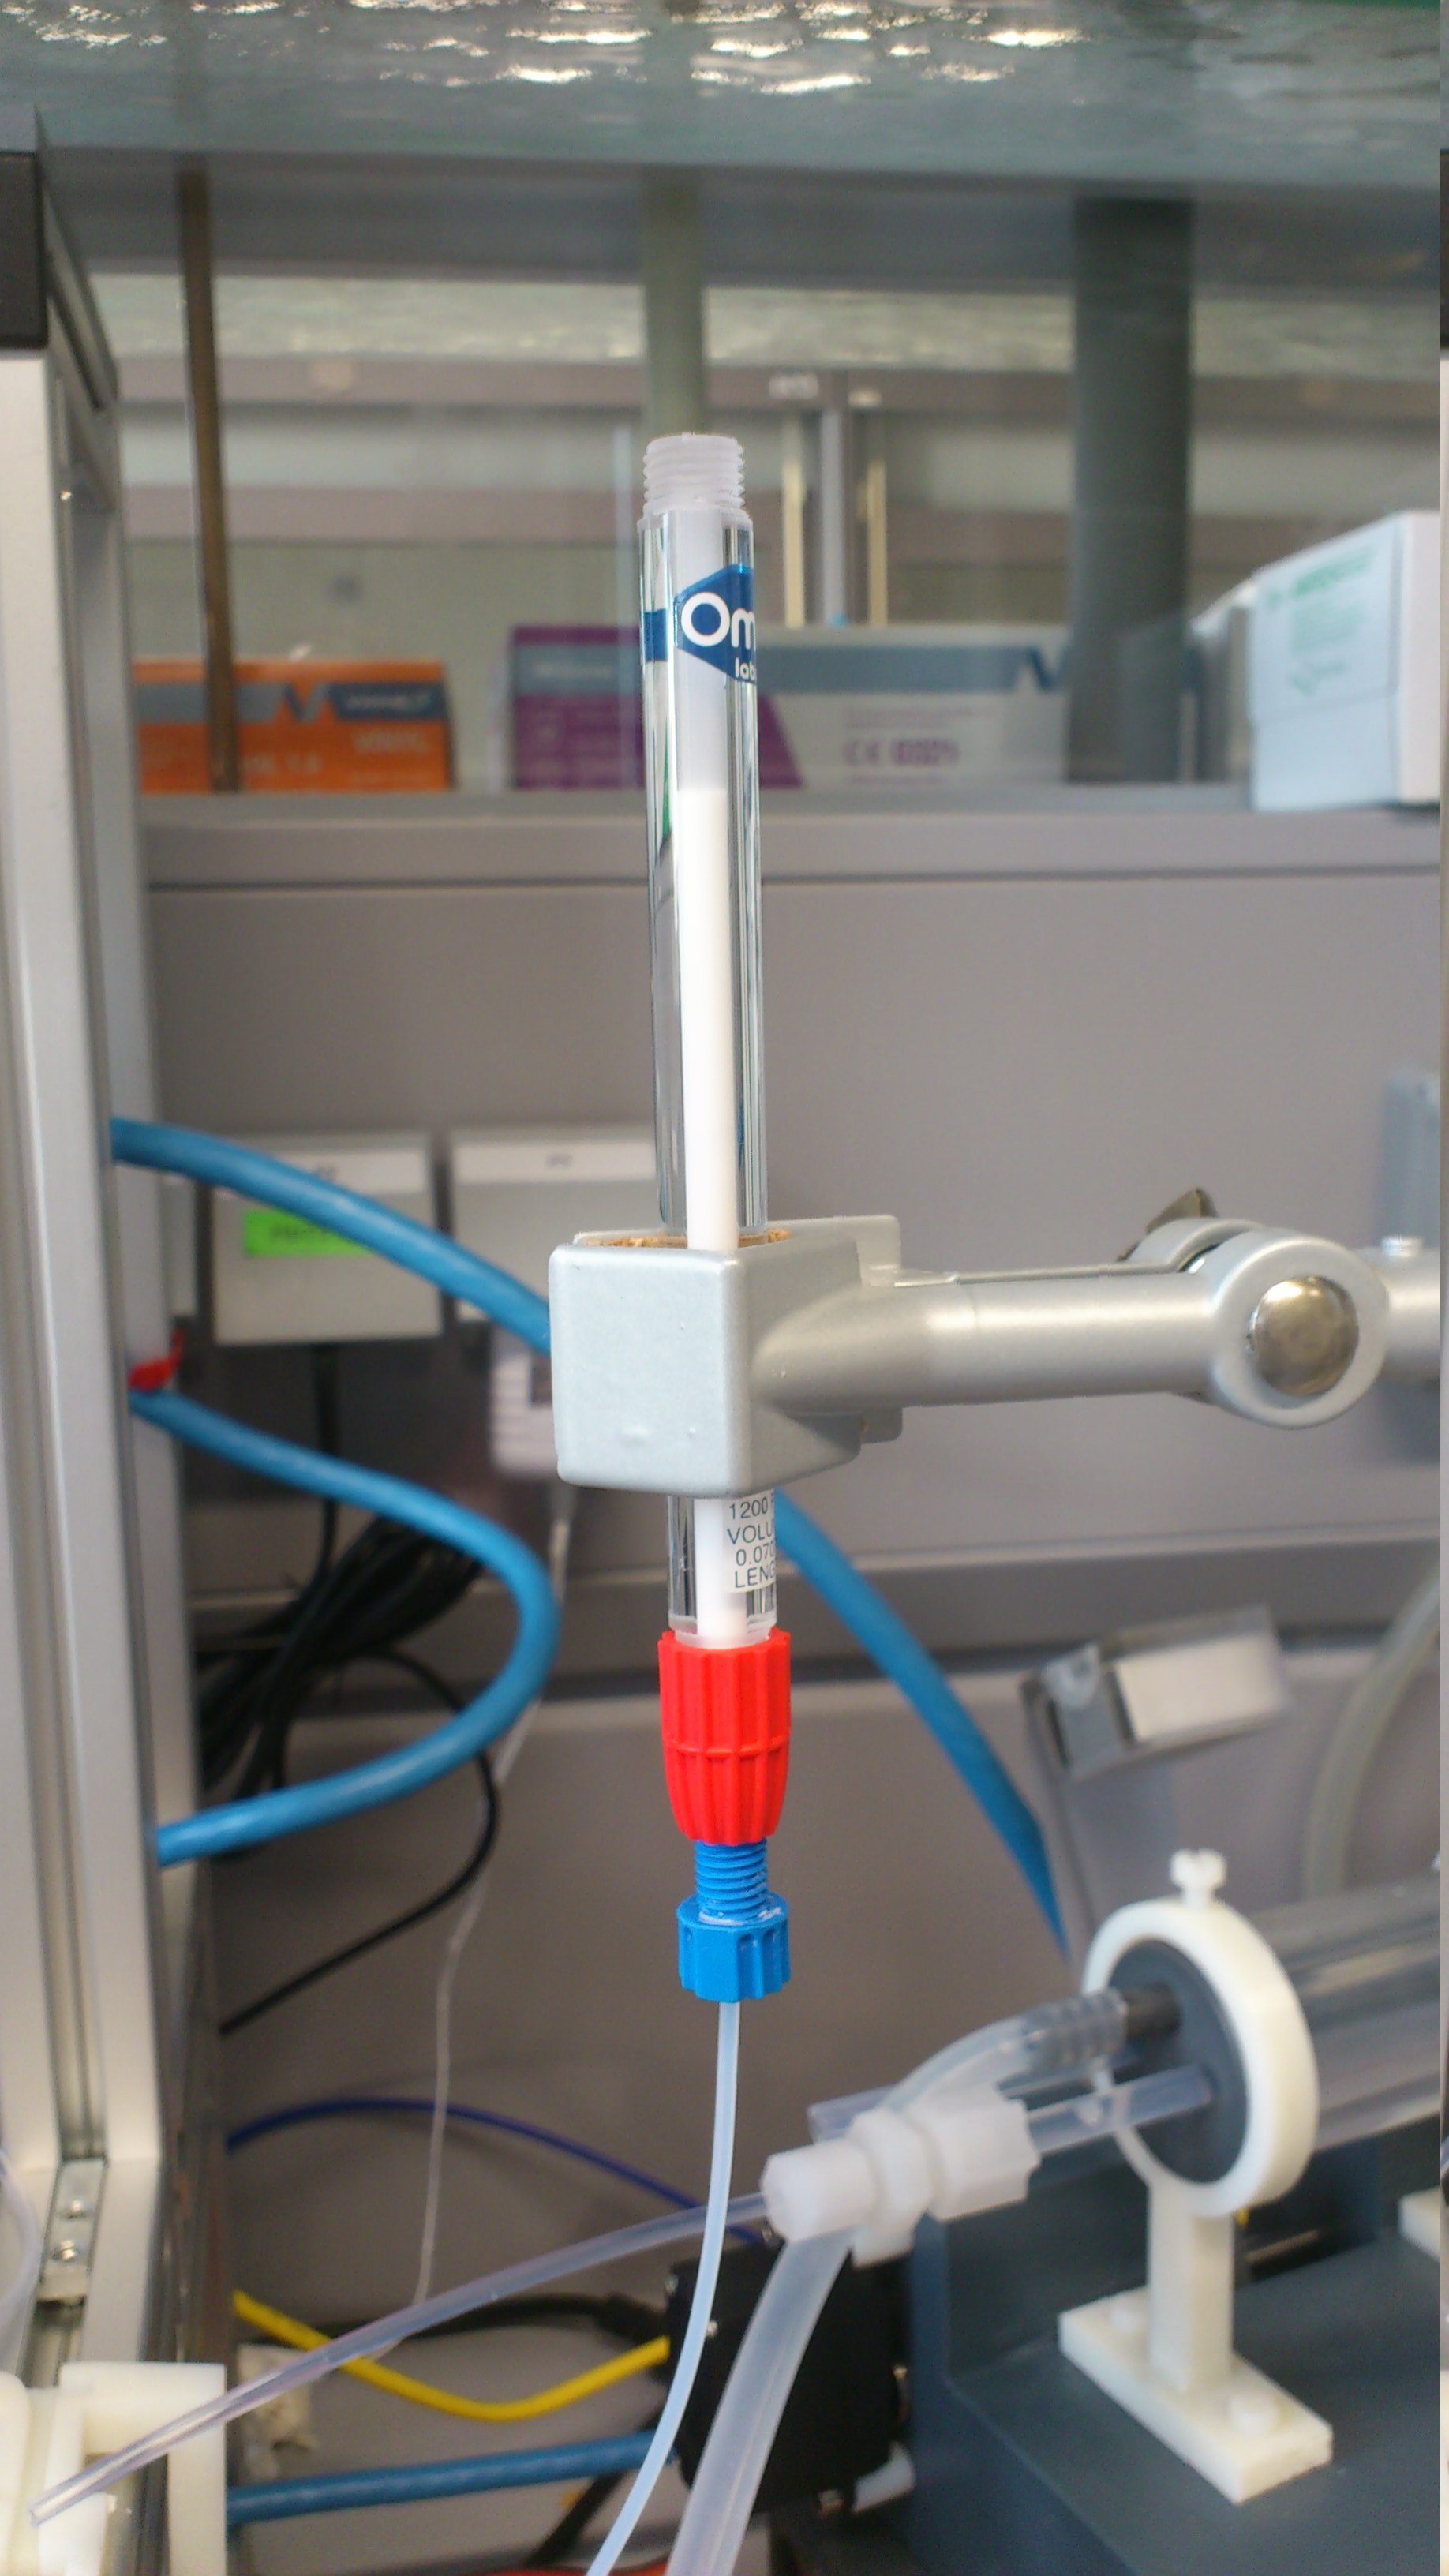
\includegraphics{figures/Column_Packing_Column.jpg}}
                %\caption{Column}\label{fig:Column}
        \end{subfigure}
        \\
        
        \caption[Column packing setup]{Column packing setup; left side: CETONI neMESYS control station (1), column (2) and syring pump (3); right side: Column packed with \gls{pmma} matrix material }
        \label{fig:Packing_Setup_Column}
  \end{figure}  




% \begin{figure}[H]
% \centering
% 
% \scalebox{0.30}{\includegraphics{Bioreactor_real.png}}
% \caption{Photobioreactor with 37 light cylinders for the cultivation of microalgae
% \label{fig: Bioreactor_real}
% }
% \end{figure} 
% 
% \begin{figure}[h]
% 		\centering
%           \begin{subfigure}{0.49\textwidth}
%                   \flushleft
%                   \scalebox{0.30}{\includegraphics{Bioreactor_Geometry.png}}
%                   \caption{Lateral view of the photobioreactor}\label{fig:Bioreactor_Geometry}
%           \end{subfigure}
%         \begin{subfigure}{0.49\textwidth}
%                 \flushright
%                 \scalebox{0.32}{\includegraphics{Bioreactor_cross_section.png}}
%                 \caption{Cross section of the photobioreactor}\label{fig:Bioreactor_cross_section}
%         \end{subfigure}
%         \\
%         
%         \caption{Structure of the photobioreactor with 37 light cylinders}
%         \label{fig:Bioreactor}
%   \end{figure}  


\subsection{Chromatographic system}
\label{subsec:chrom_sys}
For the compression of the packed bed within the column and the execution of the retention experiments an Äkta purifier \gls{fplc}-system from GE Healthcare (Buckinghamshire, England) was used. For all connections tubings with an inner diameter of 0.25\,mm (PEEK tubings blue, GE Healtcare Bio-Sciences AB, Uppsala, Sweden) were used to achieve high resolution peaks. The samples were injected via a sample loop with a total volume of 100\,\textmu m. The experiments were conducted with ultra-pure water as solvent and a constant flow rate. An inline UV flow cell was used to continuously measure the absorbance of the liquid at a wavelength of 280 nm and to transmit the data to the computer. A conductivity flow cell was used to measure the conductivity of the passing solution. For further analysis the samples were collected by a fraction collector. The regulation of the \gls{fplc}-system and the analysis of the transmitted data was realized by the software Unicorn. The experimental setup is shown in Figure \ref{fig:  }.
%%%%%%%%%%%%%%%Include Figure of ÄKta and Fraction collector%%%%%%%%%%%%%%%%%%%%%

\subsubsection{Chromatographic system with a Helmholtz coil}
\label{subsubsec:helm_coil}
For all experiments a Helmholtz coil was used to create a stable homogeneous magnetic field around the column. The Helmholtz coil consists of an assembly of four coils with the distance D between each other. The whole length of the four coils was based on the length of the column. The other calculated dimensions of the Helmholtz coil can be found in Table \ref{table:Helmholtz_coil}. The Helmholtz coil was constructed so that for a current of 2\,A a magnetic field of 14\,mT was created. The coil was also designed to be used in an ultrasonic bath. The technical drawing for the construction of the used Helmholtz coil is shown in Figure \ref{fig:Helmholtz_coil}\\  
The Helmholtz coil was included in the chromatographic system as shown in Figure \ref{fig: ???}. The coil was connected to a power amplifier (19 Z/500, FG Elektronik) to increase the electrical signal and therefore the magnetic field within the coil. The square wave signals were generated by a function generator (Rigol DG1022, RIGOL Technologies Inc., Beijng, China). The adjustment of the magnetic flux density was achieved by the regulation of the electric current measured with a digital multimeter(MY64, Mastech Group LLC., CA, USA).   

\begin{table}[H]
\centering
\caption[Dimensions of the Helmholtz coil]{Calculated dimensions of the Helmholtz coil}
\label{table:Helmholtz_coil}
\begin{tabular}{ll}\hline
Parameter &  Value \\
\hline\hline
 number of turns in each coil n & 300 \\
 filling factor F & 0.73\\
 diameter of copper wire $d_{D}$ & 0.70\,mm\\
 coil depth & 10\,cm\\
 distance between coils D & 3.3\,cm \\
 inner radius $R_{i}$ & 3.0\,cm\\ 
 outer radius $R_{a}$ & 4.58\,cm\\
 mean/average radius $R_{m}$ & 3.79\,cm\\
 \hline
\end{tabular}
\end{table}


\begin{figure}[H]
		\centering
          \begin{subfigure}{0.49\textwidth}
                  \flushleft
                  \scalebox{0.40}{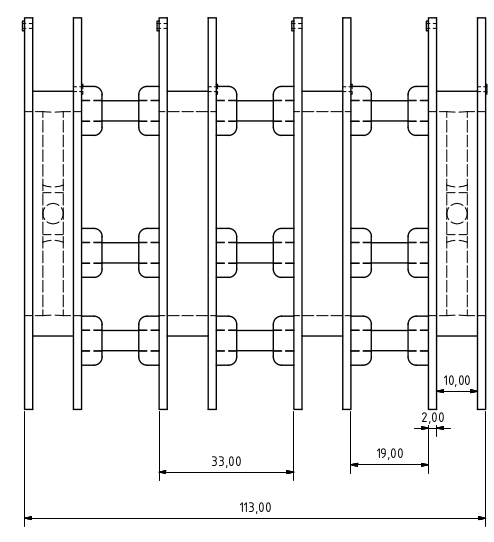
\includegraphics{figures/Helmholtz_Coil_Full.png}}
                  \caption{Side view of the Helmholtz coil}\label{fig:Coil_Full}
          \end{subfigure}
        \begin{subfigure}{0.49\textwidth}
                \flushright
                \scalebox{0.5}{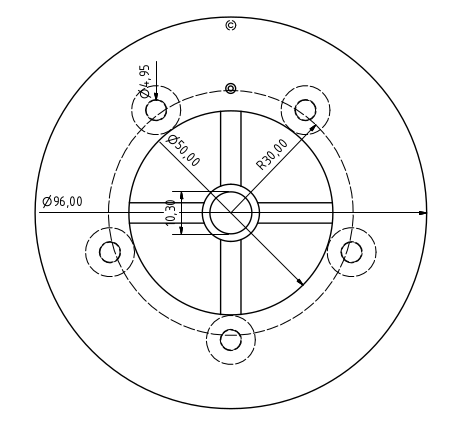
\includegraphics{figures/Helmholtz_Coil_Top.png}}
                \caption{Top view of the Helmholtz coil}\label{fig:Coil_Top}
        \end{subfigure}
        \\
        
        \caption[Technical drawing of the Helmholtz coil]{Technical drawing of the Helmholtz coil with length specifications in mm }
        \label{fig:Helmholtz_coil}
  \end{figure}  

\subsection{Experimental procedures}
\label{subsec:Exp_Pro}
All experiments were programmed and regulated using the control software Unicorn 5.20 (GE Healthcare Life Sciences). Before each injection the column was washed with 2\,ml of ultra-pure water to remove remaining nanoparticles from the previous injection. To achieve comparability and reproducibility all experiments were conducted with the same method, except for the fractionation and saturation experiments ,for which a separate method was created. All experiments were done in triple determination. \\
Before each experiment series the quality of the column packing was controlled. For this purpose a one percent acetone solution was injected and the asymmetry of the  resulting UV peak analyzed. For a packing with \gls{pmma} an asymmetry between 1 and 2 and for a packing with the TruForm particles an asymmetry between 1 and 1.5 was considered tolerable. For deviating asymmetry values the column was emptied and repacked. After each experiment series the column was demagnetized with the help of a degaussing coil (Entmagnetisierer EM-60, MAGNET-PHYSIK Dr. Steingroever GmbH, Cologne, Germany). Afterwards the column was washed until no significant change in the UV signal was perceived anymore. To clean the filters of the column and reduce the back pressure a change between up- and down-flow was applied while washing when necessary. Once a pressure of 50\,bar was reached the filters were replaced. The blocked filters were regenerated by storing them for 24 hours in oxcalic acid with a concentration of 250\,g/l on a stirrer plate with the lowest heating level.

\subsubsection{Flow rate optimization}
\label{subsubsec:Flow_rate}
In a first step the flow rate was optimized for each matrix material. For this purpose flow rates of 0.1\,ml/min, 0.2\,ml/min and 0.5\,ml/min were tested. The nanoparticle suspension was injected with a volume of 100\,\textmu l and the above mentioned method (see Section \ref{subsec:Exp_Pro}) run with the corresponding flow rates. The resulting UV peaks were analyzed for their asymmetry and reproducibility. Also the comparability with the results from \cite{AndreMaster} was taken into consideration.  

\subsubsection{Retention of magnetic nanoparticle suspension}
\label{subsubsec:Ret_nanopart_method}
The main objective of this experiments was to asses the retention of the magnetic nanoparticles through a magnetized packed bed. The magnetization of the packed bed was achieved by the Helmholtz coil described in Section \ref{subsubsec:helm_coil}. The homogeneous magnetic field within the coil was created by a power amplifier connected to a function generator, which generated an alternating current with a square wave signal. The power amplifier was used to change the electric signal and thereby vary the magnetic flux density. For all experiments a flow rate of 0.5\,ml/min and magnetic flux densities between 0\,mT and 17\,mT were used. \\
The magnetic field could be influenced by the variation of the frequency, duty cycle and amplitude. A constant magnetic field was produced by setting the high and low state to the closest values possible. The smallest difference achievable with the used function generator was 4\,mV. Therefore a high level value of 400\,mV and a low level value of 396\,mV was used to approximate a direct current (see Figure \ref{fig:waveform}). To investigate the impact of an alternating magnetic field the low level was set to -\,400\,mV wereas the high level stayed at 400\,mV. To simulate a magnetic field being turned on and off a low level value of 0\,mV was chosen. For the matrix material \gls{pmma} all described variations were applied with the frequencies 100\,mHz and 1000\,mHz . For the matrix material Stark and TruFrom only the constant and on/off fields with frequencies of 100\,mHz, 500\,mHz and 1000\,mHz were tested. The duty cycle, the ratio of the high period to the total period of the square wave, was set to 50\,\% for all experiments. An exception was an experiment with the TruForm particles were the off phase was reduced to 20\,\%.

\begin{figure}[h]
\centering

\scalebox{0.60}{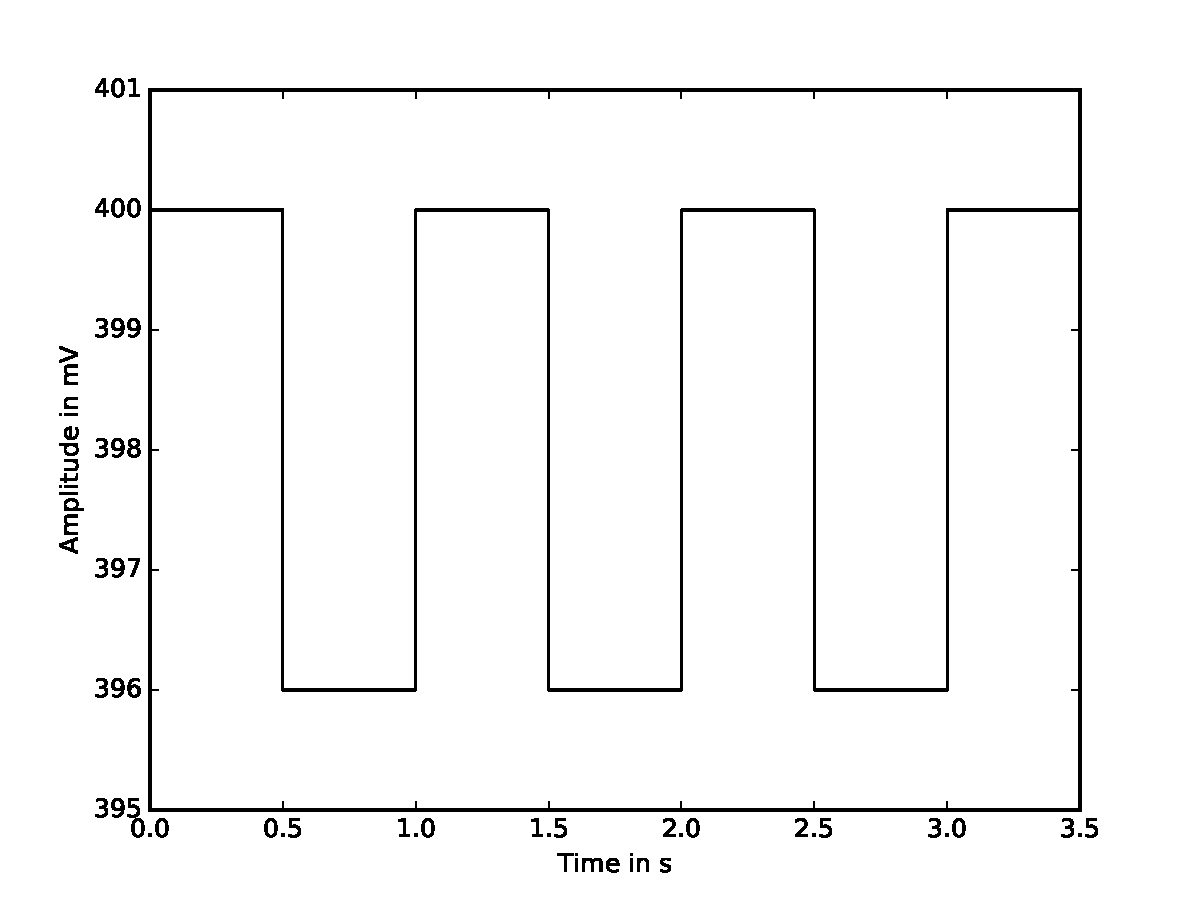
\includegraphics{figures/waveform.pdf}}
\caption[Example of a square wave signal]{Example of a square wave signal used for the generation of a constant magnetic field with a frequency of 1\,Hz, a high level of 400\,mV and a low level of 396\,mV
\label{fig:waveform}
}
\end{figure}


In addition saturation experiments were conducted with the TruForm material. For those experiments the column was first washed with 1\,ml and no magnetic field, next the sample solution was injected and the constant magnetic field was turned on. The magnetic field was held till the column was washed with 2\,ml. The cycle was repeated till no further change in the UV peak could be observed. The experiment was conducted twice, once with an used and once with a new filter. A magnetic flux density of 17\,mT was used for the saturation experiments.\\
In order to evaluate the influence of the nanoparticle concentration on the retention behaviour, Chemagen nanoparticel suspension was diluted 1:100, 1:150 and 1:200. The dilutions were tested with TruForm matrix material and a constant magnetic field. The micromod nanoparticle suspensions were also only used for experiments with the TruForm matrix material and a constant magnetic field.\\
For further analysis the third peak of each triple determination was fractionated and collected in 1.5\,ml Eppendorf tubes. A Unicorn method was written to start the fractionation as soon as an increase in the UV signal was detected. As fraction volume 200\,\textmu l was chosen. The fractionation was stopped as soon as the UV signal sank below 0.1\,mAu. 
 

%%%%%%%%%Tabelle mit Parametern ?%%%%%%%%%%%%%%%%%%%%%%%%%%%%%%%%%%%%%%%%%%%%%%%%%
 

\subsection{Analytical methods}
\label{subsec:ana_met}
 For the characterization of the matrix materials and the nanoparticle suspensions several different analytical methods were used. The particle size distribution was determined either by dynamic light scattering, light micrsocope or under the \gls{esem} described in Sections \ref{subsubsec:part_dist_meas}, \ref{subsubsec:light_mic} and \ref{subsubsec:ESEM}. The method for the determination of the magnetic properties is described in Section \ref{subsubsec:Mag_char}. For characterization of the magnetic field within the Helmholtz coil a Hall effect sensor was used (see Section \ref{subsubsec:Hall_eff}).   
 
 
\subsubsection{Measurement of particle size distributions}
\label{subsubsec:part_dist_meas}
For the determination of the particle size distribution two different measurement devices were used. The matrix materials were analyzed with an CIS 100-S particle sizer (Galai, Migdal Haemek, Israel). The measurement system combines two analytical techniques, namely laser obstruction time analysis and dynamic image analysis to analyze both the size distribution and shape factors of the sample. For the laser obstruction time measurement a helium-neon laser with a wavelength of 600\,nm rotates with a constant frequency and interacts with particles in the sample solution. Each scanned particle temporarily blocks the path of the laser beam to the corresponding photo diode, which registers the time of transition. The obstruction time in combination with the frequency is then related to the particle diameter \cite{neis1997particle}. Additionally dynamic image analysis is used to determine the particle shape parameters. With this combination spherical and non-spherical particles in a range between 0.1\,\textmu m to 3,600\,\textmu m can be measured. For each sample a three-fold determination was conducted, with a length of 60\,s for each measurement cycle. In addition the reproducibility of the measurement was verified by the measurement software. As sample preparation a spatula tip of the matrix material was mixed with 2\,ml of ultra-pure water. Of this suspension 1500\,\textmu l were filled into a cuvette. If necessary the sample was further diluted with ultra-pure water. During the measurement period the suspension was continuously mixed with a pipette (Eppendortf Research \textsuperscript{\textregistered} plus (blue), Eppendorf AG, Hamburg, Germany) to ensure homogeneity. \\
\\
For the determination of the particle size distributions of the magnetic nanoparticle suspensions and the collected nanoparticle fractions (see Section \ref{subsubsec:Ret_nanopart_method}) a Zetasizer Nano ZSP (Malvern Instruments, Malvern, England) was used. The nanoparticle stock suspensions were diluted 1:100 in ultra-pure water, while for the fractions no further dilution was necessary. The Chemagen nanoparticle solution was measured in filtered and unfiltered form (see Section \ref{subsec:Mag_nanoparticles}), whereas the micromod particles were not filtered at all. For each measurement 50\,\textmu l of the sample was pipetted into a quarz cuvette and put into the Zetasizer. For all samples a triple determination was conducted. The size measurement was performed by dynamic light scattering. Particles scatter the light from a helium-neon laser with a wavelength of 633\,nm creating a fluctuation in the detected scattering intensity over time. This fluctuation is due to the Brownian motion, which leads to diffusion of particles at a speed related to their size and temperature. From the intensity changes a correlation function is generated from which the diffusion coefficient is deducted. The particle size distribution is then calculated with the Stokes-Einstein equation \cite{berne2000dynamic}. Particle sizes could be measured in the range of 0.3\,nm to 10\,\textmu m \cite{Zetasizer}. For the evaluation only particles in the nanometer size range were considered. In order to reduce the influence of contaminations, either leaked matrix material or dust, within the samples, all particles with a size of over 1\,\textmu m were not included in the size distributions.

\subsubsection{Environmental scanning electron microscope}
\label{subsubsec:ESEM}
The particle shape, size and surface properties were characterized with an \gls{esem} (XL 30-FEG, Philips, Amsterdam, Netherlands). \gls{esem} is a procedure in which uncoated samples can be examined with an electron beam. The samples to be analyzed were placed within the sample chamber. Then a vacuum was applied reaching pressures between 130\,Pa and 1300\,Pa. An electron beam is focused on the sample which leads to the ejection of secondary electrons from the sample surface. These secondary electrons are then accelerated towards the electric field of an detector. The detected signal is converted into an image of the sample. With this method it is possible to magnify the samples by a factor of 50 up to 5100 \cite{danilatos1993introduction}.     
\gls{esem} measurements were used for the characterization of the TruForm matrix material. As sample preparation a defined quantity of the matrix material was put on a sample holder. No further sample preparation was needed.

\subsubsection{Light microscope}
\label{subsubsec:light_mic}
The characterization of the \gls{pmma} matrix material was conducted with the help of a VHX-5000 digital microscope system (Keyence, Osaka, Japan). A 500 frames per second camera captures image data with different focus positions and generates high resolution images on an attached monitor. By variation of the shutter speed the resolution and contrast are further increased. In addition the optimal wavelength to generate clear images is automatically selected \cite{VHX5000}. For the measurement the matrix material was suspended in ultra-pure water. A few drops of the suspension were placed on a slide and put onto the object stage. The magnification was slowly increased until a high resolution image was aquired. By measuring the distance from two neighbouring pixel on the screen dimension measurements were possible. With this method the mean diameter of the measured matrix particles was determined.    


\subsubsection{Concentration determination of the nanoparticle suspension}
\label{subsubsec:Conc_MF}
For the determination of the Chemagen nanoparticle concentration 200\,\textmu l of the particle suspension was filled into an HPLC vial. All measurements were conducted in triple determination. Before filling the empty weight of the vials was determined with a MC5 microbalance (Sartorius, Göttingen, Germany). The vials were dried for 24 hours at \SI{60}{\celsius} in a drying cabinet (drying cabinet ULE 500, Memmert GmbH, Schwabach, Germany). The vials were allowed to cool in a desiccator for 20 minutes and then weighed again. From the difference between the current and the empty weight the mass of the magnetic nanoparticles could be calculated. With the calculated mass and the used suspension volume the concentration could be determined.  


\subsubsection{Magnetization determination of the matrix materials and nanoparticle suspension}
\label{subsubsec:Mag_char}
The characterization of the magnetic properties of the matrix materials was performed with an \gls{agm} (Micromag 2900, Princeton Measurments Corp, Princeton, USA). As sample preparation a defined amount of matrix material was given onto a strip of adhesive tape and hermetically sealed with another piece of tape. The sample was then placed onto a cantilevered rod including a piezoelectric element, magnetized by a dc field and overlaid by an oscillating magnetic field gradient. Through the  oscillating magnetic field gradient the sample experiences an alternating force  which is proportional to the magnitude of the field gradient and the magnetic moment of the sample. This force deflects the sample rod within the magnetic field which leads to a voltage output of the piezoelectric element. With a variation of the alternating magnetic field strength the voltage signals can be converted into a magnetization curve \cite{flanders1988alternating}. The magnetization within the magnetization curve was normalized with the mass of the used sample. Before the actual measurements, the \gls{agm} was calibrated with a nickel standard. From the hysteresis loop the magnetic properties of the materials could be extracted. On all samples a threefold determination was performed.    

\subsubsection{Analysis of the magnetic flux density}
\label{subsubsec:Hall_eff}
The magnetic flux density within the Helmholtz coil was measured with a Hall effect sensor (FH 31/4, MAGNET-PHYSIK Dr. Steingroever GmbH, Cologne, Germany). The Hall effect sensor consists of a thin rectangular p-type semiconductor material on which a constant current is applied. When the sensor is placed in a magnetic field perpendicular to the current the electrons are deflected towars one edge of the sensor. The result is a potential difference that develops between the upper and lower edge of the conductor which is referred to as the Hall voltage. The Hall voltage is proportional to the applied current and the magnetic flux density \cite{svoboda2004magnetic}.\\%%%%%V=-(I*B)/(e*rho*t) 
The magnetic flux density of the Helmholtz coil was measured for different currents in six different positions along the symmetry axis. The resulting flux density was then compared to the calculated values for the Helmholtz coil (see Section \ref{subsubsec:helm_coil}). 


\subsection{Evaluation methods}
\label{subsec:Eval}
For the evaluation of both, the particle size distribution and the retention experiments, evaluation routines were written in python. Wherever possible the same evaluation methods as in \cite{AndreMaster} were applied to ensure comparability. 

\subsubsection{Graphical evaluation}
\label{subsubsec:Graph_eval}
In order to compare the results from the particle size distribution measurements, the D-values D10, D50 and D90 were determined. D50 is defined as the diameter where half of the particles are smaller than this value. Likewise 10\,\% of the population lie below the value from D10 and 90\,\% below the value of D90 \cite{merkus2009particle}. The cumulative distribution is  approximated by a least squares polynomial fit, where the solution minimizes the squared error E (see Equation \ref{eq:polyfit_er}) for the equations shown in \ref{eq:polyfit_eq}.  

\begin{equation}
\label{eq:polyfit_er}
\centering
E = \sum_{j=0}^{k}\vert p(x_{j})-y_{j}\vert^{2}
\end{equation}

\begin{equation}
\label{eq:polyfit_eq}
\centering
\begin{split}
x[0]^{n}p[0] + ... + x[0]p[n-1] + p[n] = y[0] \\
x[1]^{n}p[0] + ... + x[1]p[n-1] + p[n] = y[1]  \\
... \\ 
x[k]^{n}p[0] + ... + x[k]p[n-1] + p[n] = y[k]
\end{split}
\end{equation}

Where $p$ represents the polynomial coefficients, $n$ the degree of the polynomial, $y$ the y-coordinates and $x$ the x-coordinates of the sample points. The coefficient matrix of the coefficient $p$ is called Vandermonde matrix \cite{bjorck1970solution}. With this fit the D-values were calculated. 
%%%%%%%%%%%%%%%%Add Number distribution%%%%%%%%%%%%%%%%%%%%%%%%%%%%%%%%%%%%%

\subsubsection{Mathematical evaluation}
\label{subsubsec:Math_eval}
For the evaluation of the retention experiments with the magnetic nanoparticle suspensions the UV signal from the \gls{fplc}-system was used. The influence of the magnetic field was determined by a comparison of the UV peak area and retention with the retention and area of a control peak with no magnetic field applied. The area of the peak (see Equation \ref{eq:area}) provides information about the particles bound in the packed bed at a certain magnetic field strength.    

\begin{equation}
\label{eq:area}
\centering
area = \sum_{j=1}^{N}[(x_{i+1}-x_{i})(\frac{y_{i+1}+y_{i}}{2})]
\end{equation}

The first term on the right side of Equation \ref{eq:area} depicts an infinitely small interval of the volume which has flown through the column in ml, while the second term describes the average of the UV signal in mAU within the limits of x. The results were normalized by dividing the area of a peak with an applied magnetic field by the area of a standard peak without the influence of ante magnetic field. \\

%%%%%%%%%Check this find better description%%%%%%%%%%%%%%%%%%%%%%%%%%%%%%%%

The equations for the calculation of the retention of the nanoparticles are shown in the following: 

\begin{equation}
\label{eq:ret_sum}
\centering
k = k_{s} = \sum_{j=1}^{N}[(x_{i+1}-x_{i})(\frac{y_{i+1}+y_{i}}{2})(\frac{x_{i+1}+x_{i}}{2})]
\end{equation}

\begin{equation}
\label{eq:ret_comp}
\centering
retention = \frac{k}{k_{s}}
\end{equation}

In order to evaluate the influence of the retention the average of volume $(x_{i+1}+x_{i})/2$ within the infinitely small interval of $x_{i+1}-x_{i}$ was added to the area. The retention $k$ of a field under magentic influence was also normalized by the division with the retention $k_{s}$ of a standard peak.   

%%%%%%%%%%%%%%%%%%%%%%%%%%%%%%%%%%%%%%%%%%%%%%%%%%
%%%%%%%%%%%%%%%%%%%%%%%%%%%%%%%%%%%%%%%%%%%%%%%%%%
%%%%%%%%%%%%%%%%%Results%%%%%%%%%%%%%%%%%%%%%%%%%%
%%%%%%%%%%%%%%%%%%%%%%%%%%%%%%%%%%%%%%%%%%%%%%%%%%
%%%%%%%%%%%%%%%%%%%%%%%%%%%%%%%%%%%%%%%%%%%%%%%%%%


\chapter{Results and Discussion}8
\label{chap:chap_res}

\section{Simulation results}
\section{Experimental results}


%\include{sections/evaluation}
%% LaTeX2e class for student theses
%% sections/conclusion.tex
%% 
%% Karlsruhe Institute of Technology
%% Institute for Program Structures and Data Organization
%% Chair for Software Design and Quality (SDQ)
%%
%% Dr.-Ing. Erik Burger
%% burger@kit.edu
%%
%% Version 1.1, 2014-11-21

\chapter{Conclusion}
\label{ch:Conclusion}


\glsaddall

%% --------------------
%% |   Bibliography   |
%% --------------------

%% Add entry to the table of contents for the bibliography
%\bibliographystyle{agsm}
\cleardoublepage
\phantomsection
\addcontentsline{toc}{chapter}{Bibliography}
\printbibliography%[omitnumbers=true]

%% ----------------
%% |   Appendix   |
%% ----------------
\appendix
%% LaTeX2e class for student theses
%% sections/apendix.tex
%% 
%% Karlsruhe Institute of Technology
%% Institute for Program Structures and Data Organization
%% Chair for Software Design and Quality (SDQ)
%%
%% Dr.-Ing. Erik Burger
%% burger@kit.edu
%%
%% Version 1.1, 2014-11-21


\iflanguage{english}
{\chapter{Appendix}}    % english style
{\chapter{Anhang}}      % german style
\label{chap:appendix}

\section{ }
\label{sec:app:}

\textbf{2 Cylinder const speed BC}
\begin{figure}[H]
		%\centering
            \begin{subfigure}{0.49\textwidth}
                  \flushleft
                  \scalebox{0.42}{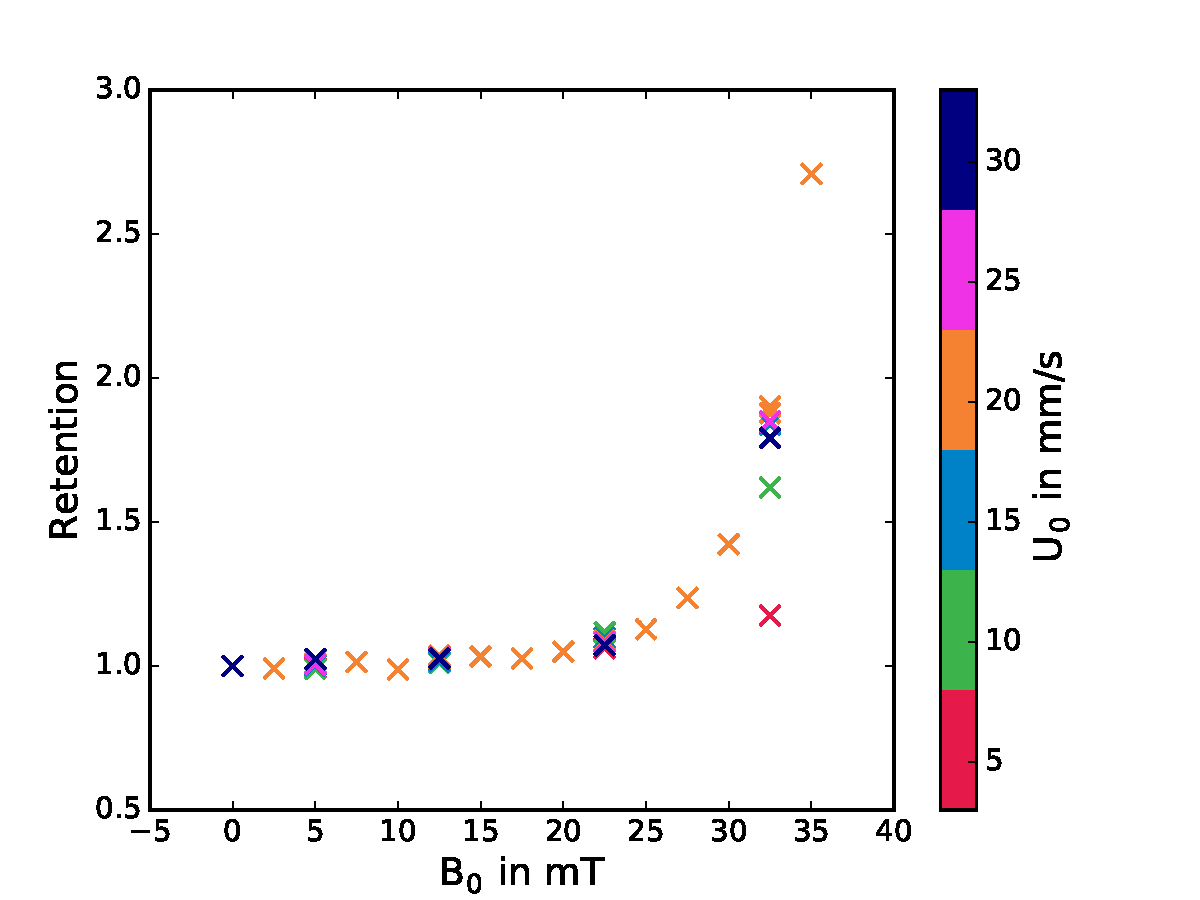
\includegraphics{figures/B0_Rp_30_U0_var_2Cylinder_constBC.pdf}}
                  \caption{Results for $R_{p}$=30\,nm and $U_{0}$ variable}\label{subfig:tw_constBC_U0_var}
          \end{subfigure}\hfill
        \begin{subfigure}{0.49\textwidth}
                \flushright
                \scalebox{0.42}{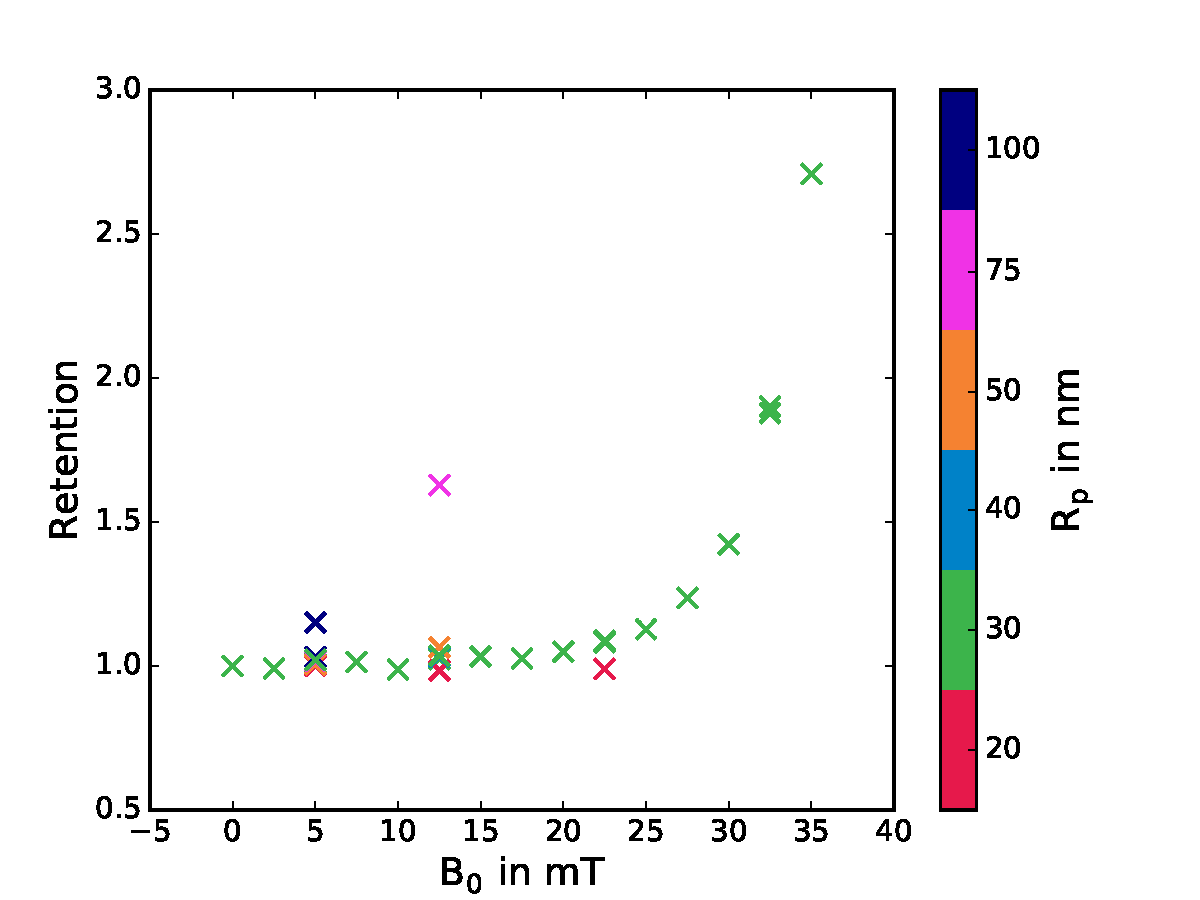
\includegraphics{figures/B0_Rp_var_U0_20_2Cylinder_constBC.pdf}}
                \caption{Results for $R_{p}$ variable and $U_{0}$=200\,\textmu m/s}\label{subfig:tw_constBC_Rp_var}
        \end{subfigure}
        \\       
          \caption[Parameter study results of the simulated retention of nanoparticles on two wires with a constant velocity boundary condition at the channel walls]{Parameter study results of the simulated retention of nanoparticles on two wires with a constant velocity boundary condition at the channel walls: the retention is plotted against the magnetic flux density $B_{0}$ in mT of the external applied magnetic field, the colorbar indicates the values of the varied parameter while the other parameters where held constant; the retention was calculated by the division of the measured residence time by the residence time for 0\,mT at the same conditions}
        \label{fig:tw_param_res_constBC}
  \end{figure}
        
\textbf{4 Cylinder const speed BC}
\begin{figure}[H]
		%\centering
            \begin{subfigure}{0.49\textwidth}
                  \flushleft
                  \scalebox{0.42}{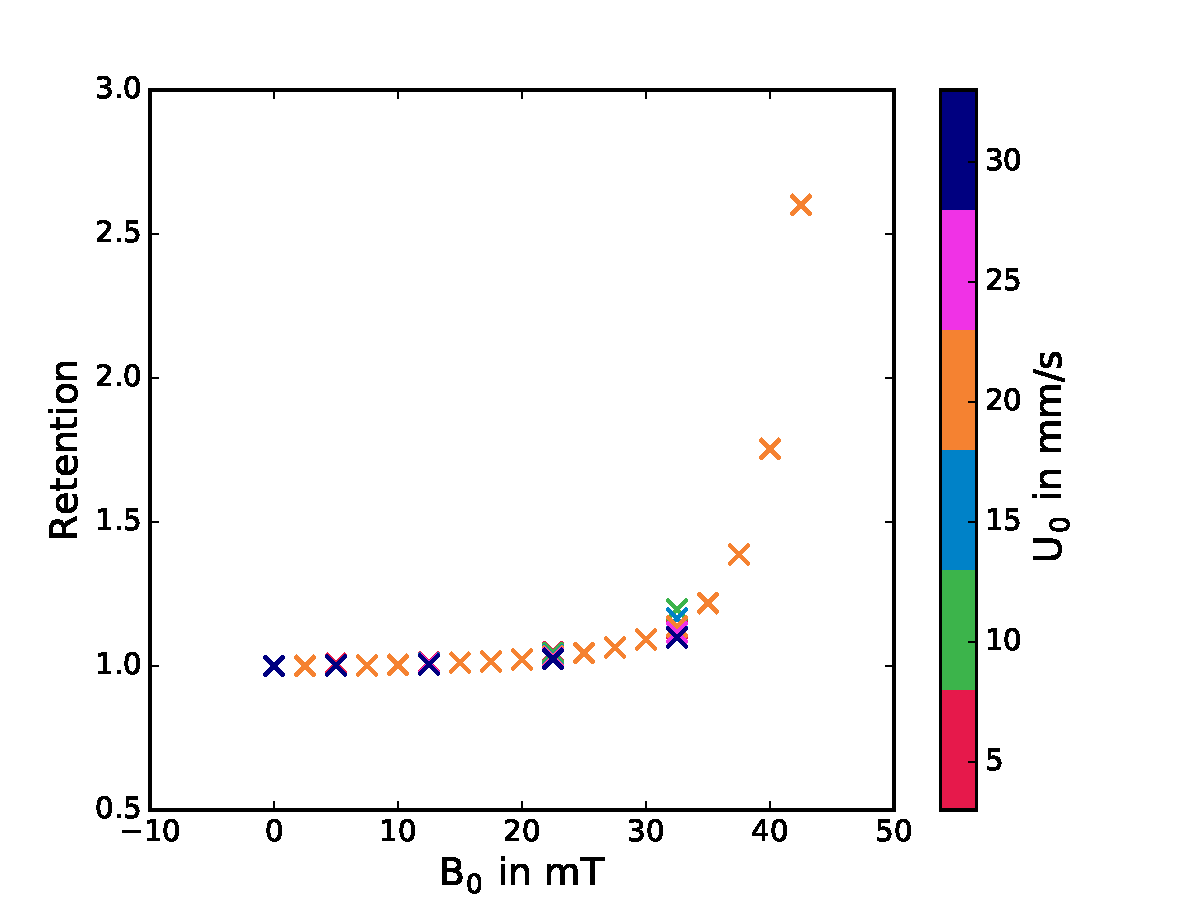
\includegraphics{figures/B0_Rp_30_U0_var_4Cylinder_constBC.pdf}}
                 \caption{Results for $R_{p}$=30\,nm and $U_{0}$ variable}\label{subfig:fw_constBC_U0_var}
          \end{subfigure}\hfill
        \begin{subfigure}{0.49\textwidth}
                \flushright
                \scalebox{0.42}{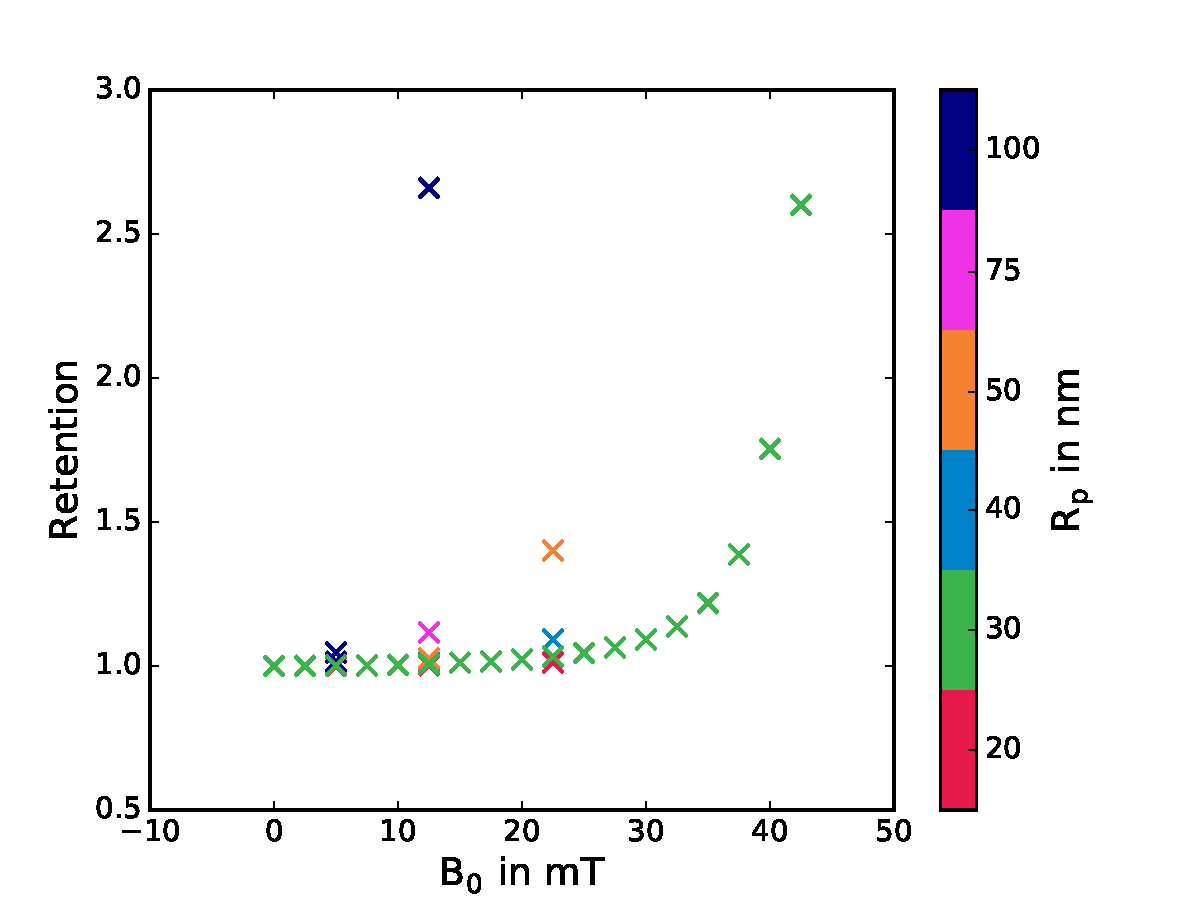
\includegraphics{figures/B0_Rp_var_U0_20_4Cylinder_constBC.pdf}}
                 \caption{Results for $R_{p}$ variable and $U_{0}$=200\,\textmu m/s}\label{subfig:fw_constBC_Rp_var}
        \end{subfigure}
        \\
        
          \caption[Parameter study results of the simulated retention of nanoparticles on four wires with a constant velocity boundary condition at the channel walls]{Parameter study results of the simulated retention of nanoparticles on four wires with a constant velocity boundary condition at the channel walls: the retention is plotted against the magnetic flux density $B_{0}$ in mT of the external applied magnetic field, the colorbar indicates the values of the varied parameter while the other parameters where held constant; the retention was calculated by the division of the measured residence time by the residence time for 0\,mT at the same conditions}
        \label{fig:fw_param_res_constBC}
  \end{figure}
        

        
\begin{figure}
		\centering
            \begin{subfigure}{0.49\textwidth}
                  \flushleft
                  \scalebox{0.42}{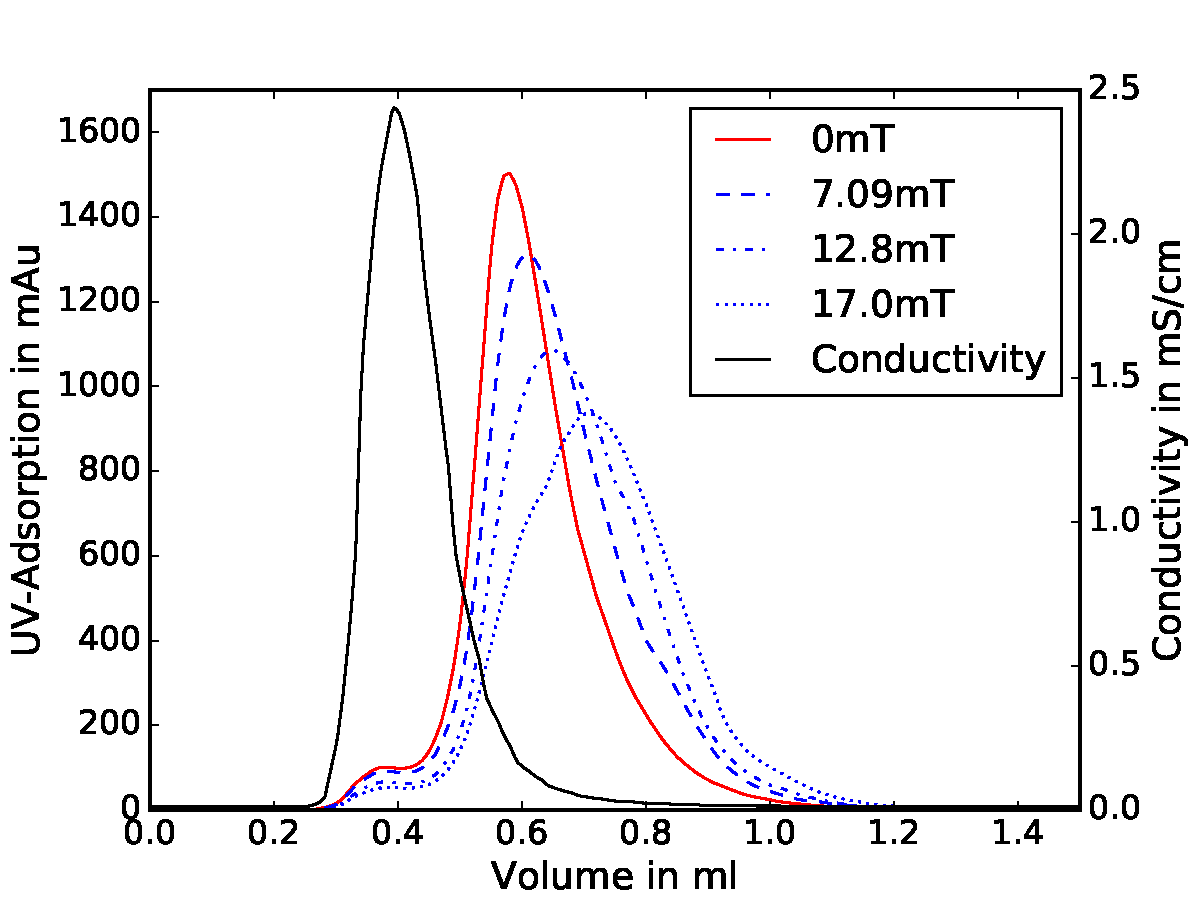
\includegraphics{figures/MF100_chemagen.pdf}}
                  \caption{}\label{subfig:sw_periodicBC_Rw_var}
          \end{subfigure}\hfill
          \\
            \begin{subfigure}{0.49\textwidth}
                  \flushleft
                  \scalebox{0.42}{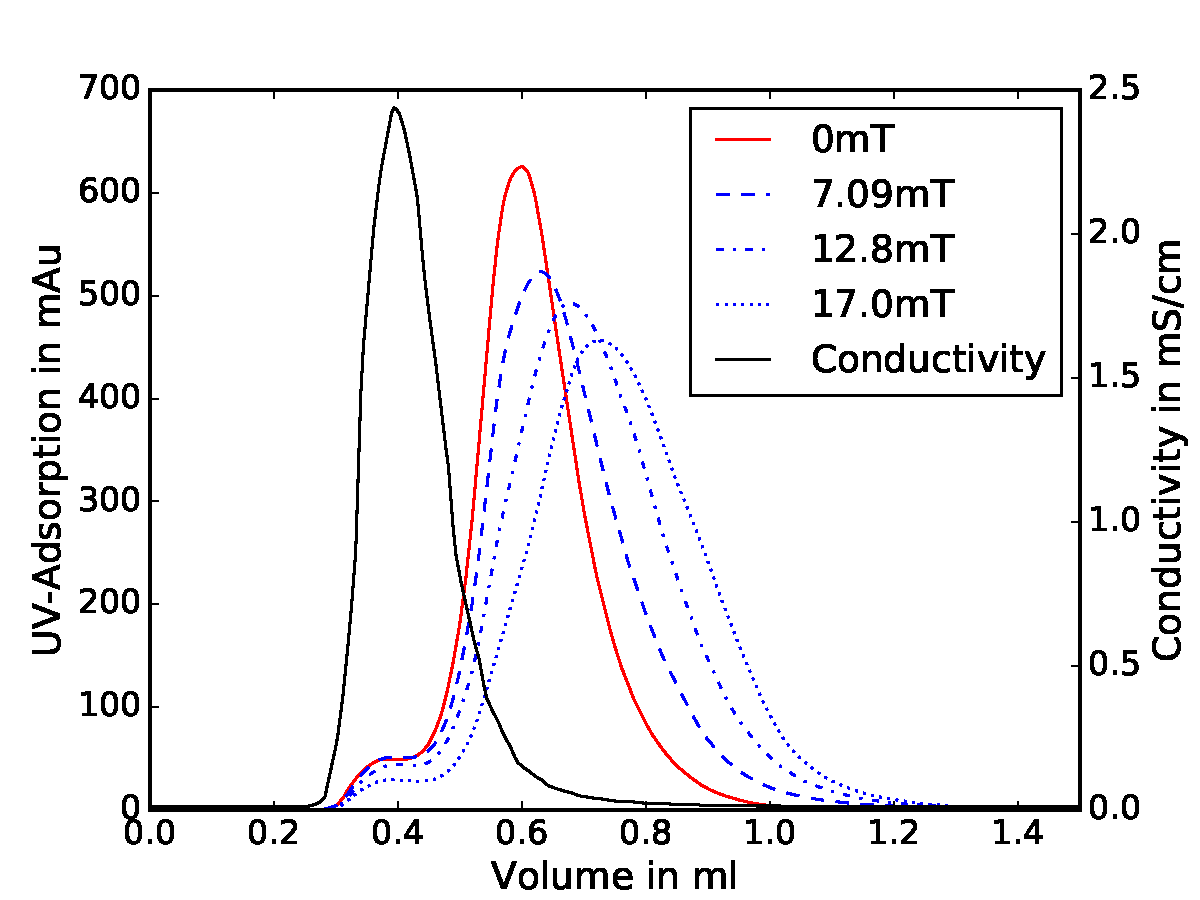
\includegraphics{figures/MF150_chemagen.pdf}}
                  \caption{}\label{subfig:sw_periodicBC_U0_var}
          \end{subfigure}\hfill
        \begin{subfigure}{0.49\textwidth}
                \flushright
                \scalebox{0.42}{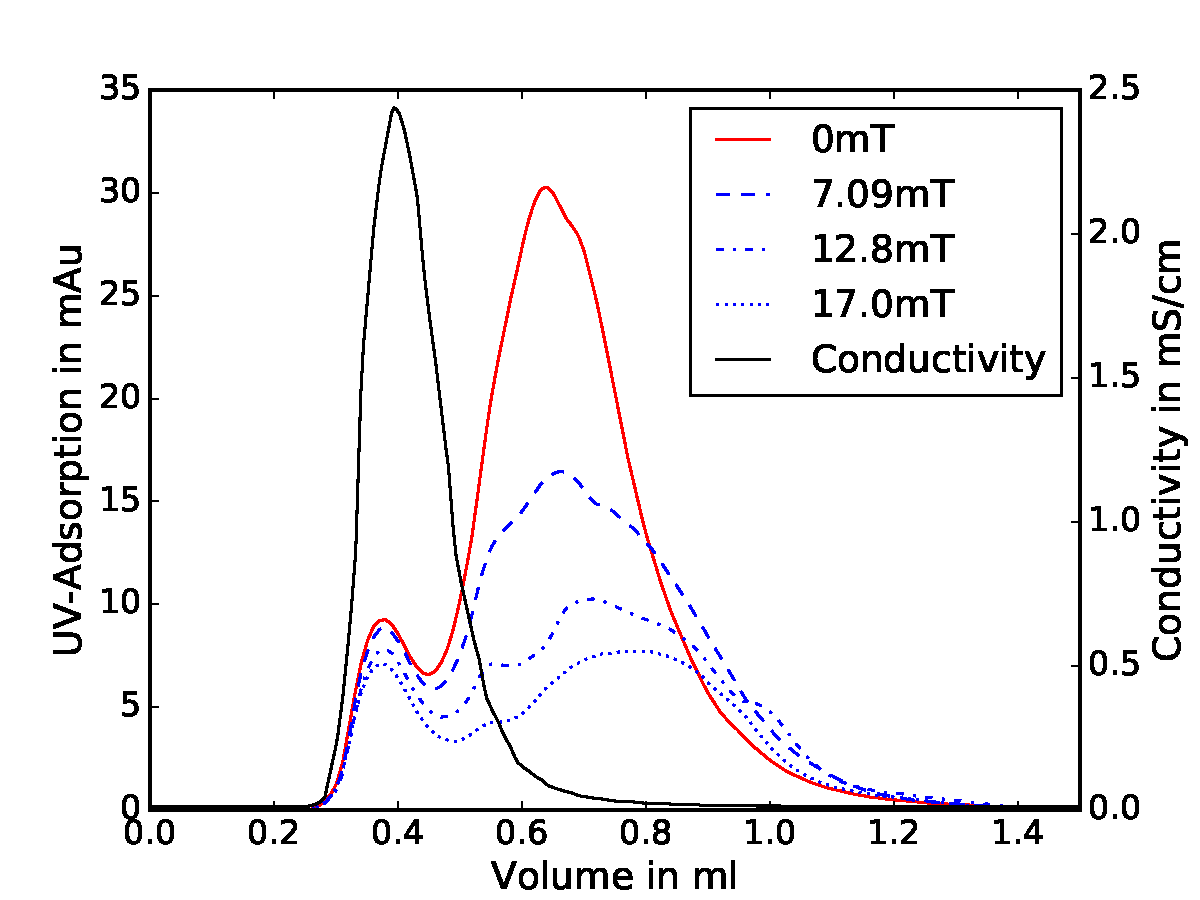
\includegraphics{figures/MF200_chemagen.pdf}}
                \caption{}\label{subfig:sw_periodicBC_Rp_var}
        \end{subfigure}
        \\
        
        \caption[]{}
        \label{fig:diff_conc_chemagen_peaks}
  \end{figure}        
		
\setcounter{figure}{0}
		


\end{document}
